\documentclass[review]{elsarticle}
\usepackage{lineno,hyperref}
\usepackage{color}
\usepackage{amsmath,amsfonts,amssymb,esvect,ulem}
\usepackage{float}
\usepackage{graphicx}
\usepackage{epsfig}

\usepackage{epstopdf}
\usepackage{subcaption}
%\usepackage{subfigure}
\modulolinenumbers[5]

\journal{Journal of Computational Physics}


%\setlength\parindent{0pt} % Removes all indentation from paragraphs
%\renewcommand{\vec}[1]{\ensuremath{\boldsymbol{#1}}}
\renewcommand{\labelenumi}{\alph{enumi}.} % Make numbering in the enumerate environment by letter rather than number (e.g. section 6)
\newcommand{\px}{\frac{\partial}{\partial x}}
\newcommand{\st}{\sigma_\mathrm{t}}
\newcommand{\pxt}{\frac{\partial^2}{\partial x^2}}
\newcommand{\stt}{\st^2}
\newcommand{\dst}{\frac{\partial\st}{\partial x}}
\newcommand{\pn}{P$_N$}
\newcommand{\dn}{D$_N$}
%\newcommand{\pnqt}{P$_N$QT}
%\newcommand{\pnqs}{P$_N$QS}
\newcommand{\tp}[1]{TP$_{#1}$}
\newcommand{\ppz}{\partial_x}%{\frac{\partial}{\partial x}}
\newcommand{\ppzt}{\frac{\partial^2}{\partial x^2}}
\newcommand{\psii}[1]{\phi_\ensuremath{{#1}}}
\newcommand{\vp}[1]{\vec{\phi}^{({#1})}}
\newcommand{\sn}{S$_N$}
%%%%%%%%%%%%%%%%%%%%%%%
%% Elsevier bibliography styles
%%%%%%%%%%%%%%%%%%%%%%%
%% To change the style, put a % in front of the second line of the current style and
%% remove the % from the second line of the style you would like to use.
%%%%%%%%%%%%%%%%%%%%%%%

%% Numbered
%\bibliographystyle{model1-num-names}incidation

%% Numbered without titles
%\bibliographystyle{model1a-num-names}

%% Harvard
%\bibliographystyle{model2-names.bst}\biboptions{authoryear}

%% Vancouver numbered
%\usepackage{numcompress}\bibliographystyle{model3-num-names}

%% Vancouver name/year
%\usepackage{numcompress}\bibliographystyle{model4-names}\biboptions{authoryear}

%% APA style
%\bibliographystyle{model5-names}\biboptions{authoryear}

%% AMA style
%\usepackage{numcompress}\bibliographystyle{model6-num-names}

%% `Elsevier LaTeX' style
\bibliographystyle{elsarticle-num}
%%%%%%%%%%%%%%%%%%%%%%%
\newcommand{\zh}{ZrH$_x$}
\newcommand{\e}[1]{\ensuremath{\times 10^{#1}}}
\newcommand{\TAMU}{Texas A\&M University}
\newcommand{\ddxcs}{\sigma(E'\to E,~\mu)}
\newcommand{\sigmat}{\sigma_\mathrm{t}}
\newcommand{\sigmas}{\sigma_\mathrm{s}}
\newcommand{\sigmaa}{\sigma_\mathrm{a}}
%\newcommand{\sb1}{\hat{\sigma}_\mathrm{b}}
\begin{document}

\begin{frontmatter}

\title{Moment Closures Based on Minimizing the Residual of the \pn~Angular Expansion in Radiation Transport}%The Transient P$_N$\ (\tp{N})\ Model: an Accurate P$_N$~Closure for Radiation Transport}
%\tnotetext[mytitlenote]{Fully documented templates are available in the elsarticle package on \href{http://www.ctan.org/tex-archive/macros/latex/contrib/elsarticle}{CTAN}.}

%% Group authors per affiliation:
\author[mymainaddress]{Weixiong Zheng}
\ead{zwxne2010@tamu.edu}
%% or include affiliations in footnotes:
%\author[mymainaddress,mysecondaryaddress]{Elsevier Inc}
%\ead[url]{www.elsevier.com}

\author[mymainaddress]{Ryan G. McClarren\corref{mycorrespondingauthor}}
\cortext[mycorrespondingauthor]{Corresponding author}
\ead{rgm@tamu.edu}

\address[mymainaddress]{Nuclear Engineering, \TAMU,~College Station, TX 77843-3133}

\begin{abstract}
	In this work we present  two new closures for the spherical harmonics (\pn) method in slab geometry transport problems. Our approach begins with an analysis of the squared-residual of the transport equation where we show that the standard truncation and diffusive closures do not minimize the residual of the \pn~expansion.  Based on this analysis we derive two models, a moment-limited diffusive (ML\dn) closure and a transient \pn~(\tp{N}) closure that attempt to address shortcomings of common closures.  The form of these closures is similar to flux-limiters for diffusion with the addition of a time-derivative in the definition of the closure.  Numerical results on a pulsed plane source problem, the Gordian knot of slab-geometry transport problems, indicate that our new closure outperforms existing linear closures.  Additionally, on a deep penetration problem we demonstrate that the \tp{N}~closure does not suffer from the artificial shocks that can arise in the M$_N$ entropy-based closure. Finally, results for Reed's problem demonstrate that the \tp{N}~solution is as accurate as the P$_{N+3}$ solution. {We further extend the T\pn\ closure to 2D Cartesian geometry. The line source test problem demonstrates the model effectively damps oscillations and negative densities.}

%	There are well-known drawbacks to simulating time-dependent particle transport problems with spherical harmonics, also known the as \pn\ method. One of the reasons is that the particles are modeled using a finite numbers of speeds forming artificial waves in the solution. Efforts has been put to correct this issue by modifying the \pn\ closure historically. Though some of them, such as \dn\ and M$_N$,\ improve the solution somehow in the sense of dampening the artificial waves, not very many methods retains high accuracy of the flux profile in short-time transient.
%	
%	We start from a novel functional analysis of residual of spherical harmonics approximation for ordinary \pn\ closure and conventional diffusive closure and find an interpretation of their failure in simulating radiation transport in short time transient. And indicated by the analysis, we find out adding two flux limiters into the \dn's closure would potentially reduce the residual of the approximation to transport and enhance the accuracy.
%	
%	A pulse test is performed by using \pn,\ \dn\ and the new nonlinear closures and comparisons indicate the nonlinear closure presents more accurate results in short-time transient in a pulse test problem than zero closure and diffusive closure. We therefore name this model ``Transient \pn (\tp{N})".\ We also observe that the nonlinear treatment sharpen the wavefront of particle compared with \dn.\ Steady state test indicates that the new nonlinear closure results in more accurate scalar flux profile than \dn.
%	
%	Extending the nonlinear closure to multi-D application is ongoing and promising for time-dependent transport problems. Also, extension to multi-physics problems are worth investigating.
\end{abstract}

\begin{keyword}
	Spherical harmonics closures\sep Radiation transport
\end{keyword}

\end{frontmatter}

\linenumbers

\section{Introduction}
%\subsection{Background and Motivation}
%{
%\begin{itemize}
%	\item Various methods and their natures and why pn
%	\item pn deficiency and what people do
%	\item what we do and the synopsis of this paper.
%\end{itemize}}
The Boltzmann equation is used to describe particle transport in several applications, e.g.\ neutron transport \cite{glasstone}, thermal radiative transfer \cite{pomraning1973equations}, rarefied gas dynamics \cite{Grad:1949wi}, and charged-particle transport in semiconductors \cite{markowich2012semiconductor}, to name a few. Solving the transport equation is challenging due to the seven-dimensional phase space. In this work we deal with a simple transport model with a linear collision operator, though our methods could be extended to more complicated transport processes. 

For the angular discretization a commonly used method is the discrete ordinates method (\sn),\ which solves the transport equation for several selected discrete angles. However, there are physical situations where \sn\ encounters difficulties. One example is in multi-dimensional applications, when the medium weakly interacts with the particles. In this case the solution along each ordinate are not coupled, which leads to the well-known ``ray effects" in the solution \cite{Mathews:1999uv}. Ray effects can remain present even when the number of discrete angles is large \cite{Morel:2003vt}. %One may have to use more angles in order to mitigate the ray effects and obtain accurate results.

Another approach is to use a truncated spherical harmonics expansion (\pn)\ on the angular variable. The \pn~method is a spectral method in angle based on a linear expansion of angular flux, yielding a hyperbolic system of partial differential equations (PDEs) for the expansion coefficients, or equivalently, the moments. For smooth angular dependence, the method has spectral convergence. Also, the spherical harmonics expansion are rotationally invariant, in contrast to \sn,\ thereby avoiding ray effects.

Nevertheless, in time-dependent problems, truncating the basis at a finite order $N$\ and assuming moments with higher orders to be zero\footnote{The resulting closure is referred to as zero closure in this paper.} causes the solution  to approximate the radiation as a finite number of waves moving with different speeds determined by the eigenvalues of the coefficient matrix of spatial derivative terms. These wave speeds are less than the real speed of the particles \cite{brunner_app_rad_trans,mccfpn09,McClarren:2008cq}.\ The artifacts in the solution that arise from the discrete wave speeds are referred to as ``wave effects". Wave effects can induce oscillations and negativity densities in the solution \cite{mccfpn09,coryentropy}. Though one could increase the order of the  \pn\ approximation to mitigate the oscillations, for a finite order of approximations, there are always certain physical situations where negative particle densities can occur \cite{McClarren:2008hu,mccdissertation}.

Here we briefly summarize the recent efforts to improve the \pn~method.\ A linear diffusive closure was developed independently by Schafer, Frank and Levermore \cite{levermoredn}\ for general orders of expansion and by Kyeong and Holloway specifically for P$_3$ \cite{p3qs}. Solutions using this closure demonstrated faster convergence to the transport solution. Additionally, Olson introduced a modification of the coefficients for highest moment equations as introduced in the P$_{1/3}$\ equation so the maximum speed of the waves is fixed to be the correct particle speed \cite{Olson:2000vq}. %Yet, these two linear closure do not provide boundedness of the solution which will potentially yield oscillations and negativities in certain situations. 

Other work has investigated closures based on the solution of an optimization problem based on an entropy (called the M$_N$ method) \cite{cory_hauck_closures,brunnerentropy} or the positivity of the particle density (called the positive \pn~method) \cite{ppn}. These methods do have some benefits, such as guaranteed positive solutions. The numerical solution of the resulting equations using high-order expansions is computationally prohibitive because an optimization problem must be solved for each spatial degree of freedom in each time step. Additionally, the optimization problem resulting from high-order M$_N$ expansions is ill-conditioned. Furthermore, in some test problems, entropy-based closures can cause artificial  shocks to develop in the solution  \cite{cory_hauck_closures,brunnerentropy}. 

Inspired by the usage of artificial viscosity in hydrodynamics, Hauck and McClarren introduced a filtering process, which is interpreted as artificial viscosity in angle \cite{mccfpn09,McClarren:2010de}.\ The basic idea is to introduced a new spherical harmonics basis which introduces dampening on high order moment coefficients. Though it outperforms conventional closures, it cannot guarantee positivity of the particle density because it is a linear closure. Radice et al\ introduced a new form of the filter that was independent of the mesh and time step \cite{fpn_radice} and applied it to radiative transfer problems in astrophysics. {On the other hand, it is also found that the filtering introduced by McClarren and Hauck does not smoothly transition to zero when increasing the \pn\ angular order. Ahrens et al\ introduce a cubic filter to address the problem\cite{ahrens_fpn}.}

% it is not perfect in the sense that the filtering strength depends on mesh sizes and does not have a limit. Also, there is no hint whether this closure can ensure the positivity. Since the filtering can also be interpreted as artificial scattering in angle\cite{mccfpn09}, which enforces the independent particles to communicate with each other, Olson directly introduced empirical artificial scattering cross sections into the \pn\ systems which efficiently dampened the oscillations\cite{olson_report}. Another filtered \pn\ work by Radice et al\ is based on similar principle\cite{fpn_radice}.

In this work, we introduce two new closures that are designed to improve the residual of \pn~expansions in 1D slab geometry. We start off defining a functional based on the angularly-integrated squared residual. By examining the minimizer of the functional, we arrive at two nonlinear closures based on the residual. Both approaches write the closure as a rational function times the derivative of a moment, similar to flux limited diffusion. We analytically demonstrate one closure will bound the magnitude of highest moment by the scalar flux. The other closure is a modification that involves the zeroth moment of the angular flux. Further, we numerically demonstrate the high accuracy of the closures in a problem with strong wavefronts. On Reed's problem \cite{reed_1971} we show that our new closure converges to the transport solution faster than diffusive closures or the standard truncation.
%We also examined the solution for one of the nonlinear closures on steady state problems and reveal that the closure forms a sharp wavefront and fix the over diffusive feature of the conventional diffusive closure. Also, with $N$\ moments, the nonlinear closure result in an accuracy comparable to diffusive closure with $N+2$\ moments in Reed's problem\cite{reed_1971}. Also, in the process of the functional analysis, we present a new explanation of the performance of conventional \pn\ and the diffusive closure in time dependent problems.

\section{Derivation of the Method}
\subsection{Error functional derivation of the P$_N$ equations}\label{s:derive}
We begin with an energy-independent transport equation for neutral particles in slab geometry given by \cite{glasstone} 
\begin{equation}\label{te}
\frac{1}{v}\frac{\partial\psi(x,\mu,t)}{\partial t}+\mu \frac{\partial}{\partial x} \psi(x,\mu,t)+\sigma_\mathrm{t}\psi(x,\mu,t)=q(x,\mu,t).
\end{equation}
In this equation the angular flux of particles is given by $\psi(\mathbf{r},\mathbf{\Omega},t)$ with units of particles per area per time. Our notation is standard with $x \in \mathbb{R}$ being the spatial variable, $\mu \in [-1,1]$ as the cosine of the angle between the slab normal and the direction of flight, and $t$ as the time variable. The macroscopic total interaction cross-section with units of inverse length is given by $\sigmat$, and $q$ contains the prescribed source, $Q(x,\mu)$, and the scattering source:
\begin{equation} \label{eq:scat_source}
q = \frac{Q}{2} + \frac{\sigmas}{2}\phi,
\end{equation}
with the scalar flux, $\phi(x,t)$, defined as
\begin{equation} \label{eq:scalarflux}
\phi(x, t)  = \int\limits_{-1}^{1} d\mu\, \psi(x,\mu,t).
\end{equation}


In order to solve Eq.~(\ref{te}) one needs to apply discretizations in space, angle, and time.  In this work we focus on the angular discretization, in particular we will expand the angular dependence in Legendre polynomials as 
\begin{equation} \label{eq:Pn_expansion}
\psi(x,\mu,t) = \sum_{l=0}^\infty C_l \phi_l(x,t) P_l(\mu),
\end{equation}
where the Legendre polynomials are given by
\begin{equation} \label{eq:legPoly}
P_l(\mu) = {1 \over 2^l l!} {d^l \over d\mu^l } \left[ (\mu^2 -1)^l \right].
\end{equation}
Here, 
$\phi_l(x,t)$ is an expansion function, and $C_l$ is a normalization constant given by
\[ C_l = \left(\int_{-1}^{1} d\mu\,P_l(\mu) P_l(\mu)\right)^{-1}.\]
This technique is known as the $P_n$ method, and generalizes to general three-dimensional geometries by making the expansion functions spherical harmonics \cite{glasstone}.
%it, different angular discretization techniques can be applied. We restrict ourselves on spherical harmonics in the angular treatment.

The typical way that the expansion functions and normalization constants are generated is via a Galerkin procedure where one assumes a Legendre expansion of the angular flux, plugs it into the transport equation, and integrates the result against different Legendre polynomials. An alternative derivation involves defining a {error functional} measuring the difference of angular flux, $\psi$~and the spherical-harmonics-reconstructed angular flux using an expansion that is truncated beyond the  $l=N$ moment, $\bar{\psi}_N$ \cite{mccfpn09}. We define the errror functional as the integrated square of the difference between the true angular flux and the truncated expansion:
\begin{equation}\label{cstf1}
J_1(\mathbf{\Omega})=\int\limits_{4\pi}d\Omega~(\psi-\bar{\psi}_N)^2,
\end{equation}
where
\begin{equation}\label{cstf}
\bar{\psi}_N(\mathbf{\Omega})=\sum_{l=0}^N C_l \phi_l(x,t) P_l(\mu).
\end{equation}
In order to minimize the functional in Eq.~\eqref{cstf},~one forces $\partial J_1/\partial\phi_l=0$, leading to
the expansion coefficients being given by
\begin{equation}
\phi_l=\int\limits_{-1}^{1}d\mu\,\psi(x,\mu,t)P_l(\mu).
\end{equation}

%In 1D situation, the expansion degrades to Legendre expansion. The corresponding coefficient is computed by Eq.~\eqref{legendre}.
%\begin{equation}\label{legendre}
%\phi_l=\int\limits_{-1}^{1}d\mu~\psi(\mu)P_l(\mu)
%\end{equation}
Using this definition for the expansion coefficients, we take a certain Legendre polynomial and integrate it with the transport equation, Eq.~(\ref{te}), over $\mu$ to get:
\begin{equation}
\frac{1}{v}\frac{\partial}{\partial t} \phi_l+\frac{l}{2l+1}\frac{\partial\phi_{l-1}}{\partial x} +\frac{l+1}{2l+1}\frac{\partial\phi_{l+1}}{\partial x}+ (\sigma_{t} - \sigmas\delta_{l,0} )\phi_l=q_\mathrm{ext}\delta_{0,l},~l=0,1,\cdots N
\end{equation}
where $\displaystyle q_\mathrm{ext}(x)=\int\limits_{-1}^1d\mu~Q(x,\mu)$. 
This system is not closed in the sense that the equation for the $N$th moment includes the $N+1$ moment, which is not included in our truncated expansion. A common closure is to set $\psii{N+1}=0$. Thereafter, the closed \pn~equation system can be described as:
\begin{multline}\label{pne}
\frac{1}{v}\frac{\partial}{\partial t}\phi_l+\frac{l}{2l+1}\frac{\partial\phi_{l-1}}{\partial x}+\frac{l+1}{2l+1}\frac{\partial\phi_{l+1}}{\partial x}(1-\delta_{N,l})\\+(\sigma_\mathrm{t}-\sigma_\mathrm{s}\delta_{0,l})\phi_l
=q_\mathrm{ext}\delta_{0,l},~l=0,1,\cdots,N.
\end{multline}
These equations are the standard \pn\, equations.  We will now change the derivation to use a functional that minimizes the residual in the transport equation given a particular expansion.

%However, cost function in Eq.~\eqref{cstf1},~rather minimize the square error of \pn~approximated angular flux, it would not necessarily preserve a small residual for \pn~equations.

\subsection{A functional based on the squared-residual}
%\subsubsection{Rewriting \pn~system}
%To aid the discussion, we rewrite the \pn~equation such that the closure is separately listed, i.e.
%\begin{subequations}
%\begin{align}\label{pnmain}
%\frac{1}{v}\partial_t\phi_l+\frac{l}{2l+1}\frac{\partial\phi_{l-1}}{\partial x}(1-\delta_{0,l})+(\sigma_\mathrm{t}-\sigma_\mathrm{s}\delta_{0,l})\phi_l\\\nonumber
%+\frac{l+1}{2l+1}\frac{\partial\phi_{l+1}}{\partial x}=q_\mathrm{ext}\delta_{0,l},~l=0,1,\cdots,N
%\end{align}
%\begin{equation}\label{zeroclose}
%\psii{N+1}=0,
%\end{equation}
%\end{subequations}
%where the $\delta$~is the Kronecker delta function. The purpose of forming \pn~system in this way is such that we may keep the main body of system along with the paper but only change the closure equation individually.
%
%\subsubsection{A new cost function}
Rather than basing the functional on the squared difference between the expansion and the true solution, one could also measure the squared residual of the \pn~approximation as:
\begin{equation}
J(\{\psii{l'}:l'=0,\cdots\})=\int\limits_{-1}^{1}d\mu~R^2,
\end{equation}
where $R$~is the residual computed when the expanded flux to order $N$ is plugged into the transport equation with an isotropic source. For  simplicity, we consider the pure absorber problem (though removing this restriction leads to the same results) leading to the definition of residual as
\begin{align}\label{res}
R\equiv\mathcal{L}\bar{\psi}_N(\mu)-q(\mu)
=\left(\frac{1}{v}\partial_t+\mu\ppz+\st\right)\sum\limits_{l'=0}^{N}\frac{2l'+1}{2}\psii{l'}P_{l'}(\mu)-\frac{q_\mathrm{ext}}{2},
\end{align}
where the transport operator $\mathcal{L}$~is defined as:
\begin{equation}
\mathcal{L}\equiv\frac{1}{v}\partial_t+\mu\ppz+\st.
\end{equation}

In order to minimize the functional $J$, we focus on finding moment sets which make $\partial J/\partial\psii{l}=0$ for all $l$. Through this path, we could gain an insight into the impact on the residual due to the closure.

Taking the functional derivative of Eq.~\eqref{res}~leads to:
\begin{multline}\label{func}
\frac{\partial J}{\partial\psii{l}}=(2l+1)\st\int\limits_{-1}^{1}d\mu~RP_l(\mu)~+ 
(2l+1)\frac{\partial}{\partial\psii{l}}\left[\frac{\partial}{\partial x}\psii{l}\right]
\int\limits_{-1}^{1}d\mu~R\mu P_l(\mu)+\\(2l+1)\frac{1}{v}\frac{\partial}{\partial\psii{l}}\left[\frac{\partial}{\partial t}\psii{l}\right]\int\limits_{-1}^{1}d\mu~RP_l(\mu).
\end{multline}

Note that for $l\leq N$, the following identity holds%operating the residual with $\displaystyle\int\limits_{-1}^1d\mu~(\cdot)$~results in:
\begin{equation}\label{pnn}
\int\limits_{-1}^1d\mu~RP_l(\mu)=\frac{1}{v}\partial_t\phi_l+\frac{l}{2l+1}\frac{\partial\phi_{l-1}}{\partial x}(1-\delta_{0,l})+\sigma_{t}\phi_l+\frac{l+1}{2l+1}\frac{\partial\phi_{l+1}}{\partial x}-q_\mathrm{ext}\delta_{0,l}.
\end{equation}
Comparing Eq.~\eqref{pnn}~with Eq.~\eqref{pne},~one sees that the integral is equal to zero, i.e.
\begin{equation}\label{pnn2}
\int\limits_{-1}^1d\mu~RP_l(\mu)=0,\qquad l\leq N.
\end{equation}

Also, by using recurrence relation of Legendre polynomial, one has:
\begin{equation}\label{recurr}
\int\limits_{-1}^{1}d\mu~R\mu P_l(\mu)=\frac{l}{2l+1}\int\limits_{-1}^{1}d\mu~\mu P_{l-1}(\mu)R+\frac{l+1}{2l+1}\int\limits_{-1}^{1}d\mu~\mu P_{l+1}(\mu)R.
\end{equation}

Therefore, Eq.~\eqref{func}~can be rewritten as:
\begin{multline}\label{func2}
\frac{\partial J}{\partial\psii{l}}=(2l+1)\left(\st+\frac{1}{v}\frac{\partial}{\partial\psii{l}}\left[\frac{\partial}{\partial t}\psii{l}\right]\right)\int\limits_{-1}^{1}d\mu~RP_l(\mu)+\\
\frac{\partial}{\partial\psii{l}}\left[\frac{\partial}{\partial x}\psii{l}\right]
\left(l\int\limits_{-1}^{1}d\mu~RP_{l-1}(\mu)+(l+1)\int\limits_{-1}^{1}d\mu~RP_{l+1}(\mu)\right).
\end{multline}

When $l < N$,~
plugging Eq.~\eqref{pnn2}~back into Eq.~\eqref{func2} leads to:
\begin{equation}
\frac{\partial J}{\partial\psii{l}}=0, \qquad l < N.
\end{equation}
That is,  all of the P$_N$ equations minimize the squared-residual for $\phi_l$ for all $l<N$. This is why the omission of the scattering term does not affect our results: the scattering term only appears in the $l=0$ equation. It is in the $l=N$ equation where the closure enters. We will now explore what that equation tells us.
%So far, we observe the zero-value functional derivative up to Order $N-1$, as expected {Shall we talk about our expectation somewhere?}. Nevertheless, we shall be cautious with the same operation when $l=N$,~where the closure lives. 

For $l=N$,~the same substitution, omitting the algebraic process, results in:
\begin{align}\label{func3}
\frac{\partial J}{\partial\psii{N}}=(N+1)
\frac{\partial}{\partial\psii{N}}\left[\frac{\partial}{\partial x}\psii{N}\right]
\left(\int\limits_{-1}^{1}d\mu~RP_{N+1}(\mu)\right).
\end{align}
Therefore, expanding the integral term in Eq.~\eqref{func3}~gives us the final expression for the $N^\mathrm{th}$~order functional derivative:
\begin{multline}\label{func4}
\frac{\partial J}{\partial\psii{N}}=(N+1)
\frac{\partial}{\partial\psii{N}}\left[\frac{\partial}{\partial x}\psii{N}\right]
\left(\frac{1}{v}\partial_t\phi_{N+1}+\frac{N+1}{2N+3}\frac{\partial\phi_{N}}{\partial x}\right.\\
\left.+\sigma_{t}\phi_{N+1}+\frac{N+2}{2N+3}\frac{\partial\phi_{N+2}}{\partial x}\right).
\end{multline}
This equation can tell us the impact of a closure on the residual: to this equation we can substitute in a closure and see how it effects the derivative of the squared residual.

%From now on, the discussion for the theoretical part will be mainly based on Eq.~\eqref{func4}~since we realize that it is possible to observe the impacts on residual from the closures through the last functional derivative due to the fact that it contains more than one undetermined moments, which are simply ``thrown away" (zero closure) in conventional \pn~system.

\subsection{Discussion on two conventional closures}\label{s:above}
%Indicated by the analysis above, monitoring the functional deriative in Eq.~\eqref{func4}\ would provide hints whether a closure could provide accurate results in time dependent problems.

\subsubsection{Zero closure}
Introducing the zero closure ($\psii{\mathcal{M}}=0,~\mathcal{M}>N$) into Eq.~(\ref{func4}) gives the following:
\begin{equation}\label{bd}
\frac{\partial J}{\partial\psii{N}}=(N+1)
\frac{\partial}{\partial\psii{N}}\left[\frac{\partial}{\partial x}\psii{N}\right]
\frac{N+1}{2N+3}\frac{\partial\phi_{N}}{\partial x}
.
\end{equation}
This equation indicates that the squared-residual will be minimized only if the spatial derivative of $\phi_N$ is zero.  This restriction is not expected to be satisfied in general problems.

%The treatment of zero closure itself is simple due to the fact that the resulting system is linear and the idea is straightforward. Yet, Eq.~\eqref{bd}~indicates an undesirable property of zero closure: whether or not the minimal residual of \pn~approximation exists depends on the solution itself. 

\subsubsection{Diffusive closure}
Levermore et al.~suggested a diffusive closure which takes a form similar to Fick's law for the relationship between $\psii{N+1}$~and $\psii{N}$\cite{levermoredn}:
\begin{equation}\label{fick}
\psii{N+1}=-\frac{1}{\st}\frac{N+1}{2N+3}\ppz\psii{N}.
\end{equation}
They, therein, name the corresponding system D$_N$~in the sense that the closure is essentially taking the definition of diffusion to a high-order closure. Also, Oh and Holloway independently derived a low order D$_2$~method for transient problem by assuming the closed moment $\psii{N+1}$~is time-independent such that one could directly gain the Fick's law-like relationship in Eq.~\eqref{fick}\cite{p3qs}.~They name the method P$_3$QS, short for P$_3$~quasi static, because of the approximation used to find the closure. 
%\sout{As a extension, we will call diffusive closure method D$_N$ or P$_N$QS at the same time. Since we closed the system at the odd order (i.e.~$N$~is even.), which means the system will have odd numbers of equations differing from conventional \pn,~to keep the system rotationally invariant, one shall see D$_{N-1}$~and P$_N$QS are used alternatively in this paper (e.g.~D$_2$~is equivalent to P$_3$QS for time-dependent problems).} The \dn~system in this paper is closed at odd order (i.e.,\ N\ is even.) to preserve the system rotational invariance.

Substituting Eq.~\eqref{fick}~into Eq.~\eqref{func4}, we get:
%\begin{align}\label{bd2}
%\frac{\partial J}{\partial\psii{N}}=&(N+1)
%\frac{\partial}{\partial\psii{N}}\left[\frac{\partial}{\partial x}\psii{N}\right]
%\left(\frac{1}{v}\partial_t\phi_{N+1}+\frac{N+2}{2N+3}\frac{\partial\phi_{N+2}}{\partial x}\right).
%\end{align}
%
%Though the way of deriving \dn\ method is to assume the closure to be time-independent, the independency is only weakly imposed. The assumption transfer the time-dependency of closure moment, $\psii{N+1}$, to that of $\psii{N}$.~This can be seen by simply plug Eq.~\eqref{fick}~back in \eqref{bd2}:
\begin{equation}\label{bd2}
\frac{\partial J}{\partial\psii{N}}=(N+1)
\frac{\partial}{\partial\psii{N}}\left[\frac{\partial}{\partial x}\psii{N}\right]
\left(-\frac{N+2}{2N+3}\frac{1}{v}\partial_t\left(\frac{1}{\st}\ppz\psii{N}\right)+\frac{N+2}{2N+3}\frac{\partial\phi_{N+2}}{\partial x}\right).
\end{equation}
This result indicates where the \dn\, closure might be accurate. It will minimize the squared-residual when the time derivative of  $\phi_N$ is zero and when the spatial derivative of the $\phi_{N+2}$ is zero.  We cannot know for a general problem what the derivative of $\phi_{N+2}$ will be. Nevertheless, we can predict when transients have died out in a particular problem.  In such an occasion we predict that the \dn\, closure will be superior to the zero closure because the derivative of the $\phi_{N+2}$ moment impacts the residual, rather than the $\phi_N$ moment in the zero closure.

%The result in Eq.~\eqref{bd2}~is interesting: one on hand, it still preserves the solution dependency of the functional derivative, which means the closure would lead to small residual only if the solution holds high regularity in time and space; on the other hand, the derivative includes a temporal derivative of the solution, which means the functional derivative could be small when the solution varies slowly in time. The first point illustrates the why numerical results are away from exact solution in some test problems; meanwhile, the second point might indicate when the short transient passed, $\partial_t(\cdot)\sim 0$,~the solution is relatively accurate.
\subsection{Two new closures}
\subsubsection{Approximations on higher moments}
Equation ~\eqref{func4} indicates that we should seek a closure such that:
\begin{equation}\label{func5}
\frac{1}{v}\partial_t\phi_{N+1}+\frac{N+1}{2N+3}\frac{\partial\phi_{N}}{\partial x}
+\sigma_{t}\phi_{N+1}+\frac{N+2}{2N+3}\frac{\partial\phi_{N+2}}{\partial x}=0,
\end{equation}
which is equivalent to introducing a higher order \pn~approximation without changing the truncation order. The closure, leading to zero functional derivative in moment space, would potentially lead to a minimized residual of the \pn~approximation. However, this is not feasible practically since truncating at a certain order $N$~would lead to the loss of information of higher orders, e.g.~$\psii{N+2}$. The value of Eq.~\eqref{func5}~is that it indicates how one could close the system to minimize the residual in moment space.

Formally, we can rewrite Eq.~\eqref{func5} to implicitly define a closure as
\begin{equation}\label{oricl}
\psii{N+1}=-\frac{1}{\sigma_\mathrm{t}+\displaystyle\frac{\partial_t\psii{N+1}}{v\psii{N+1}}+\frac{(N+2)}{(2N+3)\psii{N+1}}\ppz\psii{N+2}}\frac{N+1}{2N+3}\ppz\psii{N}.
\end{equation}


%In order to make the system closed, one potential way is to mimic the undetermined moments using moments within the truncation order. If one assumes that the angular flux is separable in time in the following way:
%\begin{equation}\label{sep1}
%\psi(z,\mu,t)=T(t)\hat{\phi}(\mu,z)+r_t(z,\mu,t),
%\end{equation}
%where the $r_t(z,\mu,t)$~is the rest part of the separation, and the separated part is dominant, one could find:
%\begin{equation}
%\frac{1}{v\psii{N+1}}\partial_t\psii{N+1}\sim\frac{1}{v\psii{0}}\partial_t\psii{0}.
%\end{equation}
%Meanwhile, if one could assume:
%\begin{equation}\label{sep2}
%\psi(z,\mu,t)=\phi(z)\hat{U}(\mu,t)+r_z(z,\mu,t),
%\end{equation}
%where the $r_z(z,\mu,t)$~is the rest part of the separation, and the separated part is dominant, one could find:
%\begin{equation}
%\frac{(N+2)}{(2N+3)\psii{N+1}}\ppz\psii{N+2}\sim\alpha(i,j,\hat{U})\frac{\partial_x\psii{i}}{\psii{j}},
%\end{equation}
%where
%\begin{equation}
%\alpha(i,j,\hat{U})=\frac{(N+2)\displaystyle\int\limits_{-1}^1d\mu~P_{N+2}(\mu)\hat{U}(\mu,t)\cdot\int\limits_{-1}^1d\mu~P_{j}(\mu)\hat{U}(\mu,t)}{(2N+3)\displaystyle\int\limits_{-1}^1d\mu~P_{N+1}(\mu)\hat{U}(\mu,t)\cdot\int\limits_{-1}^1d\mu~P_{i}(\mu)\hat{U}(\mu,t)}.
%\end{equation}
%Hence, the resulting closure could be given by:
%\begin{equation}\label{closure}
%\psii{N+1}=-\frac{1}{\sigma_\mathrm{t}+\displaystyle\frac{1}{v\psii{0}}\partial_t\psii{0}+\frac{\alpha(i,j,,\hat{U})\partial_x\psii{i}}{\psii{j}}}\frac{N+1}{2N+3}\ppz\psii{N}
%\end{equation}
%To preserve the positivity of ``adjusted cross section", the denominator, we chose to use:
%\begin{equation}\label{closure2}
%\psii{N+1}=-\frac{1}{\sigma_\mathrm{t}+\displaystyle|\frac{1}{v\psii{0}}\partial_t\psii{0}|+|\frac{\alpha(i,j,\hat{U})\partial_x\psii{i}}{\psii{j}}|}\frac{N+1}{2N+3}\ppz\psii{N}
%\end{equation}
%
%Yet, we still need to do some compromise on $\alpha$~to make the closure function well. The $\alpha$,~if it is archivable, it would depend on the angular distribution of the flux besides the order pair $(i,j)$~one chooses. A simple modification is that one choose a constant $\alpha$~for a specific $(i,j)$. All these approximations, though does not guarantee the minimum residual, does add potentially proper modification on diffusivity of the closure to the diffusive closure.

\subsubsection{A moment-limited closure}
The closure indicated by Eq.~(\ref{oricl}) shares a similar form with diffusive closure, except, there are additional terms added to correct the closure. Though it is still a formal closure since it depends on the value of $\psii{N+1}$\ and $\psii{N+2}$, it implies adding spatial and temporal flux limiters to the diffusive closure could help minimize $\partial J/\partial\psii{N}$. Therefore, we propose the following closure:
\begin{equation}\label{ml}
\psii{N+1}=-\frac{1}{\sigma_\mathrm{t}+\displaystyle\left|\frac{\partial_t\psii{0}}{v\psii{0}}\right|+\left|\frac{\alpha\partial_x\psii{N}}{\psii{0}}\right|}\frac{N+1}{2N+3}\ppz\psii{N}.
\end{equation}

%Specifically, (0,N)~is of interest due to one of properties demonstrated below. With this order pair, the closure function is:
%\begin{equation}
%\phi_{N+1}=\frac{1}{\sigma_\mathrm{t}+\displaystyle|\frac{\partial_t\psii{0}}{v\psii{0}}|+\alpha|\frac{\partial_x\psii{N}}{\psii{0}}|}\frac{N+1}{2N+3}\ppz\psii{N}
%\end{equation}
%
%If one chooses the pair $(0,N)$~and 
A desirable feature is that if a proper $\alpha$ is used, one could prove that this form limits the magnitudes of the closure as follows:
\begin{align}
|\phi_{N+1}|=\frac{1}{\sigma_\mathrm{t}+\displaystyle\left|\frac{\partial_t\psii{0}}{v\psii{0}}\right|+\alpha\left|\frac{\partial_x\psii{N}}{\psii{0}}\right|}\frac{N+1}{2N+3}\left|\ppz\psii{N}\right|\\\nonumber
\leq \frac{1}{\displaystyle\alpha\left|\frac{\partial_x\psii{N}}{\psii{0}}\right|}\frac{N+1}{2N+3}\left|\ppz\psii{N}\right|=\frac{N+1}{\alpha(2N+3)}|\phi_0|
\end{align}

For instance, fixing $\alpha$~at $(N+1)/(2N+3)$~would result in:
\begin{equation}
|\psii{N+1}|<|\psii{0}|
\end{equation}

That is similar to the situation of limiting current to the scalar flux to stabilize the system in moment space. We, therefore, name this approach the moment-limited diffusive (MLD) closure. 

\subsubsection{A modification: transient \pn\ closure}
The moment limited closure could be modified to use $\psii{0}$, instead of $\psii{N}$ in the closure. Specifically, the modified closure is expressed as:
\begin{equation}\label{closure3}
\psii{N+1}=-\frac{1}{\sigma_\mathrm{t}+\displaystyle\left|\frac{\partial_t\psii{0}}{v\psii{0}}\right|+\left|\frac{\alpha\partial_x\psii{0}}{\psii{0}}\right|}\frac{N+1}{2N+3}\ppz\psii{N}
\end{equation}
There are two motivations for this choice. On one hand, this selection is to make a form similar to  %Since the quantity of interest is the scalar flux, $\psii{0}$,\ it makes more sense to obtain the corrected dissipation from the scalar flux than using $\psii{N}$.
a high order extension of flux-limited diffusion with an additional constraint on the temporal evolution of the solution (i.e. the $\partial_t\psii{0}$~term). Moreover, in multidimensional problems $\psii{0}$ is the only moment that is a scalar, making the extension to full spherical harmonics closures straightforward. {In contrast, extending ML\dn\ to multi-D requires individual estimates of the spatial limiters for each single $(N+1)^\mathrm{th}$\ moment equation. For instance, for MLD$_3$\ in 2D with moments generated from complex-value spherical harmonics, four different spatial limiters need estimating, and the situation is worse as $N$ is increased. This is another motivation for the simpler closure in Eq.~(\ref{closure3}).}% Increasing the angular order or spatial dimension will further vastly increase the number of estimations. It is therefore complex and prohibited in this work.}

%\sout{Since we perform similar (but not identical) operation on the closed moment as Larsen-type flux limited diffusion, we name the closure flux-limited diffusive closure. } 
To minimize the residual, the parameter $\alpha$\ would depend on the unknown angular flux distribution. For simplicity, we fix the $\alpha$~in Eq.~\eqref{closure3}~to a constant. %A simple choice working well is to choose a number from the Jacobian of \pn~system.
Though the central theme is similar to the MLD model in that one adjusts the diffusivity nonlinearly based on the solution, we have not been able to prove that the closure limits the magnitude of $\phi_{N+1}$ to be less than the scalar flux. % it is difficult to analyze the limitation it puts on the closure in analytic form.% Nevertheless, it is possible to analyze that qualitatively.

%Assuming a forward Euler time discretization is performed such that the closure is evolved using the previous moment information. In a semi-discrete scheme, the closure at time Step 1 will be formulated as:
%\begin{equation}\label{closuresemi1}
%\psii{N+1}^{(1)}=-\frac{1}{\sigma_\mathrm{t}+\displaystyle\left|\frac{1}{v\psii{0}^{(0)}}\partial_t\psii{0}^{(0)}\right|+\left|\frac{\alpha\partial_x\psii{0}^{(0)}}{\psii{0}^{(0)}}\right|}\frac{N+1}{2N+3}\ppz\psii{N}^{(0)}
%\end{equation}
%If the initial condition holds that the angular flux is isotropic (also true for zero flux scenario), which is true for the problems tested in this paper, it is true the claim that $\exists$~finite number $\beta>0$~such that $\psii{0}^{(0)}\geq\beta\psii{N}^{(0)}$. In isotropic-flux initial condition, $\psii{N}^{(0)}=0$, thus the claim is always true with $\beta=1$.
%
%Introducing the inequality to Eq.~\eqref{closuresemi1},~and take the absolute values, one shall see the following limitation on the closure at first time step:
%\begin{align}\label{closuresemi2}
%&|\psii{N+1}^{(1)}|<\frac{1}{\sigma_\mathrm{t}+\displaystyle|\frac{1}{v\psii{0}^{(0)}}\partial_t\psii{0}^{(0)}|+|\frac{\alpha\partial_x\psii{0}^{(0)}}{\psii{0}^{(0)}}|}\frac{N+1}{2N+3}|\ppz\psii{N}^{(0)}|\\\nonumber
%&<\frac{1}{\displaystyle|\frac{\alpha\partial_x\psii{0}^{(0)}}{\psii{0}^{(0)}}|}\frac{N+1}{2N+3}|\ppz\psii{N}^{(0)}|\leq\frac{1}{\displaystyle|\frac{\alpha\partial_x\left(\beta^{(0)}\psii{N}^{(0)}\right)}{\psii{0}^{(0)}}|}\frac{N+1}{2N+3}\lvert\ppz\psii{N}^{(0)}\rvert\\\nonumber
%&=\frac{N+1}{\alpha\beta^{(0)}(2N+3)}|\psii{0}^{(0)}|
%\end{align}
%
%Qualitatively, at the first time step, Eq.~\eqref{closuresemi2}~is true if and only if the angular flux is bounded by some finite value $\mathcal{B}$ (it is realizable that unbounded angular flux would cause large variations in moment space),~i.e.~$|\psi(\mu)^{(1)}|\leq\mathcal{B}^{(1)}$, so reversely, it tells us every other moment must be bounded. Somehow, this is equivalent to give the relationship between $\psii{N}$~and $\psii{0}$~at the first time step: $\exists$~a finite number $\beta^{(1)}$, such that
%\begin{equation}
%\lvert\psii{N}^{(1)}\rvert\leq\beta^{(1)}|\psii{0}^{(1)}|,
%\end{equation}
%leading to:
%\begin{equation}
%|\psii{N+1}^{(2)}|<\frac{N+1}{\alpha\beta^{(2)}(2N+3)}|\psii{0}^{(1)}|
%\end{equation}
%Similarly, one could use induction to qualitatively demonstrate that, there is always a finite number $\beta^{(\gamma+1)}$~at Step $\gamma+1$, such that
%\begin{equation}
%|\psii{N+1}^{(\gamma+1)}|<\frac{N+1}{\alpha\beta^{(\gamma+1)}(2N+3)}|\psii{0}^{(\gamma)}|
%\end{equation}
%Take the limit of zero for the time step length $\delta t$,~the discrete inequality is turned to be continuous in time, i.e.~at a certain time $t$, $\exists~0<\beta(t)<\infty$~such that:
%\begin{equation}\label{fld}
%|\psii{N+1}(t)|<\frac{N+1}{\alpha\beta(t)(2N+3)}|\psii{0}(t)|
%\end{equation}

The test results in the following sections demonstrate this modification improves the accuracy in the transients that arise when a majority of the particles in the system have not had a collision. We, therefore, name the model the transient \pn\ closure (\tp{N}).

{
\subsubsection{Closure effects on residual functional derivative}
By introducing the ML\dn\ or T\pn\ closures, the functional derivative in Eq.\ \eqref{func4}\ can be written as:
\begin{subequations}\label{func_tpn}
\begin{align}
\frac{\partial J}{\partial\phi_N}=\frac{(N+1)(N+2)}{2N+3}
\frac{\partial}{\partial\psii{N}}\left[\frac{\partial}{\partial x}\psii{N}\right]
\left(-\frac{1}{v}\partial_t\left(\frac{1}{\st+\nu}\ppz\psii{N}\right)+\frac{\nu}{\st+\nu}\ppz\psii{N}+\partial_x\phi_{N+2}\right)
\end{align}
\begin{equation}
\mathrm{MLD}_N:\quad\nu=\left|\frac{\partial_t\psii{0}}{v\psii{0}}\right|+\left|\frac{\alpha\partial_x\psii{N}}{\psii{0}}\right|
\end{equation}
\begin{equation}
\mathrm{TP}_N:\quad\nu=\left|\frac{\partial_t\psii{0}}{v\psii{0}}\right|+\left|\frac{\alpha\partial_x\psii{0}}{\psii{0}}\right|.
\end{equation}
\end{subequations}
Adding flux or moment limiters does not necessarily minimize the residual functional. In fact, Eq.\ \eqref{func_tpn}\ automatically adjusts the functional derivative based upon the solution. In occasions where the spatial derivative of the solution tends to be large, $1/(\st+\nu)$\ goes to be zero while $\nu/(\st+\nu)$\ limits to  one. Eq.\ \eqref{func_tpn}\ has the limit of \pn's functional derivative. When the solution is smooth and slowly varying in time, $\nu$\ tends to be small and Eq.\ \eqref{func_tpn}\ limits to \dn.\ 
In effect, the closures improve the \dn\, method during transients and preserve the beneficial properties of that closure in the steady limit.
%Practically, nonlinear closures do improve the solution in short-time transients. Furthermore, T\pn's\ 2D extension indicate it has much higher preconditioning and solving efficiencies. Also, the nonlinear closures have consistent results with linear closure models. All the observations might be associated with the analysis above.
}

\subsubsection{Generalization of T\pn\ models}
{
The form of the T\pn~closure is similar to the Larsen-type flux limited correction to radiation diffusion\cite{Morel:2000vh}\  with an additional time derivative term. The form of a Larsen flux limiter allows the impact of the limiter to be adjusted by making the terms in the closure weighted by a power, rather than using a linear sum.  We can perform the same adjustment to our model by writing
%In fact, similar to larsen-type flux limited diffusion, the T\pn\ closure can be generalized as the following:
\begin{subequations}
	\begin{equation}
	\psii{N+1}=-\frac{1}{\tilde{\sigma}}\frac{N+1}{2N+3}\ppz\psii{N}
	\end{equation}
	\begin{equation}\label{eq:fluxLim}
	\tilde{\sigma}=\left(\sigma_\mathrm{t}^n+\displaystyle\left|\frac{1}{v\psii{0}}\partial_t\psii{0}\right|^n+\left|\frac{\alpha\partial_x\psii{0}}{\psii{0}}\right|^n\right)^{\frac{1}{n}}
	\end{equation}
\end{subequations}
Typically, the value of $n$ is set to be one or greater, though recent work has demonstrated that there are problems where $n<1$ can give improved solutions \cite{taylor_ans12}. It is then of interest to test the effects from different powers $n$ on our closure.
	}

\subsection{Multi-D extension of T\pn\ closure}
{
%\subsubsection{\pn\ equations}
The multi-D transport equation with isotropic scattering in Cartesian geometry can be expressed as:
\begin{equation}\label{e:md_trans}
\frac{1}{v}\frac{\partial\psi(\hat{\Omega})}{\partial t}+\hat{\Omega}\cdot\nabla\psi(\hat{\Omega})+\st\psi(\hat{\Omega})=\frac{\sigmas}{4\pi}\int\limits_{4\pi}d\Omega\ \psi(\hat{\Omega})+\frac{Q}{4\pi}.
\end{equation}
In multi-D, \pn\ method is from expanding the angular flux with spherical harmonics functions $Y_l^m(\Omega)$ in angle truncated at Order $N$:
\begin{subequations}
	\begin{equation}\label{e:md_expansion}
	\psi(\hat{\Omega})=\sum\limits_{l=0}^{N}\sum\limits_{|m|=0}^{l}\phi_l^mY_l^m(\hat{\Omega}),
	\end{equation}
	\begin{equation}
	Y_l^m(\hat{\Omega})=Y_l^m(\mu,\varphi)=\begin{cases}
	\sqrt{2}C_l^m\cos(m\varphi)P_l^m(\mu),& m\geq 0\\
	\sqrt{2}C_l^{|m|}\sin(|m|\varphi)P_l^{|m|}(\mu),& m>0\\
	\end{cases},
	\end{equation}
\end{subequations}
where \[C_l^m=\displaystyle\sqrt{\frac{(2l+1)}{4\pi}\frac{(l-m)!}{(l+m)!}}.\] In a similar Galerkin procedure as in Section\ \ref{s:derive}\, one uses the expansion in Eq.\ \eqref{e:md_expansion}\ in Eq.\ \eqref{e:md_trans}\ and operate on the transport equation with $\int\limits_{4\pi}d\Omega\ {Y}_l^m(\cdot)$\ for all the angular basis functions. The result is
\begin{subequations}
	\begin{equation}
	\frac{1}{v}\frac{\partial\vec{\phi}}{\partial t}+\sum\limits_{\zeta=x,y,z}\partial_\zeta\mathbf{A}_\zeta\vec{\phi}+\mathbf{\Sigma}_\mathrm{r}\vec{\phi}=\vec{Q}
	\end{equation}
	\begin{equation}
	\mathbf{A}_{\zeta,l,m}^{l',m'}=\int\limits_{4\pi}d\Omega\ {Y}_{l}^{m}(\hat{\Omega})\Omega_\zeta Y_{l'}^{m'}(\hat{\Omega})
	\end{equation}
	\begin{equation}
	\vec{\phi}=\left(\phi_0^0,\phi_1^{-1},\cdots,\phi_1^1,\cdots,\phi_N^{-N},\cdots,\phi_N^N\right)^\top,\quad\vec{Q}=(Q,0,\cdots,0)^\top
	\end{equation}
	\begin{equation}
	\mathbf{\Sigma}_\mathrm{r}=\mathrm{diag}(\st-\sigmas,\st,\cdots,\st)
	\end{equation}
\end{subequations}
Due to symmetry, there are $(N+1)(N+2)$\ moments in 3D and $(N+1)(N+2)/2$\ relevant moments in 2D.
	}

{
\subsubsection{\dn\ equations}
The \dn\ model is identical to \pn\ up to the $(N-1)^\mathrm{th}$\ moment equations. Dropping off the time derivative terms of the $(N+1)^\mathrm{th}$\ moment equations of P$_{N+1}$\ system, one can easily find:
	\begin{equation}\label{dn_2d}
	\phi_{N+1}^m=-\frac{1}{\st}\sum\limits_{\zeta=x,y,z}\sum\limits_{l',m'}\mathbf{A}_{\zeta,N+1,m}^{l',m'}\partial_\zeta\phi_{l'}^{m'},\quad |m|\leq N+1
	\end{equation} 
Plugging Eq.\ \eqref{dn_2d}\ into the relevant moment equations up to Order N will then lead to the \dn\ system. Note that Eq.\ \eqref{dn_2d}\ illustrates that \dn\ is equivalent to adding a diffusive correction to the P$_{N-1}$\ system\cite{levermoredn}.
\subsubsection{T\pn\ closure}
It is straightforward to extend modify the \dn\ model to be T\pn\ by adding a correction term $\nu$\ to the denominator of Eq.\ \eqref{dn_2d}:
	\begin{subequations}
		\begin{equation}\label{tpn_2d}
		\phi_{N+1}^m=-\frac{1}{\st+\nu}\sum\limits_{\zeta=x,y,z}\sum\limits_{l',m'}\mathbf{A}_{\zeta,N+1,m}^{l',m'}\partial_\zeta\phi_{l'}^{m'},\quad |m|\leq N+1
		\end{equation}
		\begin{equation}\label{viscosity}
		\nu\equiv\left(\left|\frac{\partial_t\phi_0^0}{v\phi_0^0}\right|+\alpha\frac{\|\nabla\phi_0^0\|}{|\phi_0^0|}\right).
		\end{equation}
	\end{subequations}
	}

\section{Numerical Details} %Boundary conditions and semi-discrete discetizations}
{
The 1D ML\dn\ and T\pn\ closures are implemented with the diamond difference for spatial discretization and a semi-implicit scheme as detailed below. At present only T\pn\ closure is extended to multi-D applications with discontinuous Galerkin (DG) finite element method in space and semi-implicit scheme in time.
	}
\subsection{1D implementation}
For our closures the highest order moment we keep in our system is $N$ with $N$ even.  With $N$ even, there are $N$\ first-order PDEs and one second-order PDE.  This requires $N+2$ total boundary conditions or $N/2 + 1$ conditions on each boundary in 1-D. We can use the standard Marshak conditions in this case where on the left boundary we satisfy 
\begin{equation}\label{e:bdy}
\int\limits_{0}^{1}\!d\mu\,\psi_{\mathrm{inc}}^\mathrm{L}(\mu)P_l(\mu)=\sum\limits_{i=0}^{N}c_i\psii{i}-\frac{c_{N+1}}{\sigma_\mathrm{t}+\displaystyle\left|\frac{\partial_t\psii{0}}{v\psii{0}}\right|+\alpha\left|\frac{\partial_x\psii{k}}{\psii{0}}\right|}\frac{N+1}{2N+3}\ppz\psii{N}, \qquad l=1,3,..,{N+1},,
\end{equation}
where $k$ is equal to $0$ or $N$, and $\displaystyle c_i=\int_{0}^1d\mu~P_l(\mu)P_i(\mu)$. The conditions at the right boundary are the same except the integral is over $\mu\in[-1,0]$. 

For a spatial discretization we use the diamond difference method with unknowns that live at cell edges. For a uniform mesh with cell width $h$, the semi-discrete equations become 
\begin{subequations}\label{eqs:DD}
	\begin{multline}
	\frac{h}{v}\partial_t\psii{l,i}+\frac{l}{2l+1}\left(\psii{l-1,i+1/2}-\psii{l-1,i-1/2}\right)+\frac{l+1}{2l+1}\left(\psii{l+1,i+1/2}-\psii{l+1,i-1/2}\right)\\
	+h\left(\sigma_{\mathrm{t},i}-\sigma_\mathrm{s,i}\delta_{0,l}\right)\psii{l,i}=Q_{l,i}\delta_{0,l}h,\quad l=0,\cdots,N-1
	\end{multline}
	\begin{multline}
	\frac{h}{v}\partial_t\psii{N,i}+\frac{N}{2N+1}\left(\psii{N-1,i+1/2}-\psii{N-1,i-1/2}\right)+h\sigma_{\mathrm{t},i}\psii{N,i}\\
	-\frac{N(N+1)}{(2N+1)(2N+3)}\left(\frac{\partial_x\psii{N,i+1/2}}{\tilde{\sigma}_{i+1/2}}-\frac{\partial_x\psii{N,i-1/2}}{\tilde{\sigma}_{i-1/2}}\right)=0
	\end{multline}
	\begin{equation}
	\tilde{\sigma}_{i}=\sigma_{\mathrm{t,}i}+\left|\frac{\partial_t\psii{0,i}}{v\psii{0,i}}\right|+\alpha\left|\frac{\psii{k,i+1/2}-\psii{k,i-1/2}}{h\psii{0,i}}\right|,
	\end{equation}
\end{subequations}
where $k$ is either $0$ or $N$, and
\begin{subequations}
	\begin{equation}
	\partial_x\psii{l,i+1/2}=\frac{\psii{l,i+1}-\psii{l,i}}{h},
	\end{equation}
	\begin{equation}
	\psii{l,i}=\frac{1}{2}\left(\psii{l,i+1/2}+\psii{l,i-1/2}\right),\quad l=0,\cdots,N,
	\end{equation}
	\begin{equation}
	\tilde{\sigma}_{i+1/2}=\frac{1}{2}\left(\tilde{\sigma}_{i+1}+\tilde{\sigma}_{i}\right).
	\end{equation}
\end{subequations}

The time discretization we use is semi-implicit that we evaluate all terms in  Eq.~(\ref{eqs:DD})\ at time level $n+1$ (i.e., backward Euler) except $\tilde{\sigma}$, which is evaluated explicitly at level $n$. This makes each time step a linear solve.  If we implicitly update $\tilde{\sigma}$, each step would require a nonlinear solve. 
\subsection{2D T\pn\ implementation}
{
Previously, \dn\ has been discretized in space by the streamline diffusion continuous finite element method\cite{levermoredn}\ and finite volume method\cite{p3qs,cory_hauck_closures}\ in space.\ We choose a variant of the discontinuous Galerkin (DG) finite element method  in this work mainly for its preservation of the asymptotic diffusion limit. In particular, we apply the local DG (LDG)\ method, which was developed for time dependent convection-diffusion equation\cite{cockburn_ldg}:\
\begin{equation}\label{conv_dif}
\frac{\partial u}{\partial t}+\nabla\cdot\mathrm{F}(u)+\nabla a(x,y,z)\nabla u=0.
\end{equation}
%It is clear that the diffusion term will prohibit the direct use of DG method. Therefore, 
In the LDG method, one introduces an auxiliary variable $\vec{q}$,\ such that Eq.\ \eqref{conv_dif}\ can be rewritten as:
\begin{subequations}\label{ldg}
\begin{equation}\label{ldg1}
\frac{\partial u}{\partial t}+\nabla\cdot\mathrm{F}(u)+\nabla\cdot\vec{q}=0,
\end{equation}
\begin{equation}
\vec{q}=a(x,y,z)\nabla u.
\end{equation}
\end{subequations}
%It is then clear that DG method can be used by solving a larger system.
	}

{
%	Applying the LDG method to \dn\ is similar to Eqs.\ \eqref{ldg}\ that $\phi_{N+1}^{m}$\ plays the role of the auxiliary variable. %The procedure is as the following:
%%\begin{enumerate}
%%	\item[1] Formulate the P$_{N+1}$\ equation system;
%%	\item[2] Erase $\partial_t(\cdot)$\ terms for $(N+1)^\mathrm{th}$\ moment equations;
%%	\item[3] Apply DG method in space to the resulting equations.
%%\end{enumerate}
%Solving T\pn\ equations follows the same procedure except that one needs to add $\nu\phi_{N+1}^m$\ with the $\nu$\ defined in Eq.\ \eqref{viscosity}\ to the collision terms of the corresponding $(N+1)^\mathrm{th}$\ moment equations.
%Apparently, in 2D, using LDG method for \dn\ system will involve the same amount of variables as in P$_{N+1}$\ equations. 
	}
%
%{
%The discretization in time is rather consistent the same as in 1D. $\nu$\ depends on the solution and is therefore nonlinear. Current 2D implementation is on uniform rectangular mesh so we estimate the spatial limiter in the same way as in 1D using cell centered difference. The temporal limiter is estimated with the lagged cell center scalar flux from previous time steps.
%	}

%
%\subsection{Boundary conditions}
%one shall be cautious on the boundary treatment. When invoking half-range integrations of the moments (either Marshak or Mark boundary methodology), the highest order of mix-order form is even. A natural thought take $N/2$ half integrals with odd order Legendre polynomial and one integral with even order Legendre polynomial on one side of the slab. We shall see in Section~\ref{num}~that in applications with incident boundary conditions the flux profile will have unphysical discrepancy with the real solution.
%
%
%Instead, we used conventional treatment that integrating with odd order Legendre polynomials up to $N+1$ (recall we close the system at even orders, e.g. $N=2$, so we would not have $\psii{3}$ in mix-order formulation). Consistently, we need to approximate the $\psii{N+1}$~with the closure on the boundary. For instance, when closing the system at $\psii{2}$,~the Marshak boundary condition on the left side of the domain could be expressed as:
%\begin{equation}\label{e:bdy}
%\int\limits_{0}^{1}d\mu~\psi_{\mathrm{inc}}(\mu)P_l(\mu)=\sum\limits_{i=0}^{2}c_i\psii{i}-c_3\frac{1}{\sigma_\mathrm{t}+\displaystyle|\frac{\partial_t\psii{0}}{v\psii{0}}|+\alpha|\frac{\partial_x\psii{j}}{\psii{0}}|}\frac{3}{7}\ppz\psii{2},
%\end{equation}
%where $l=1,3$~and $\displaystyle c_i=\int_{\mu>0}d\mu~P_l(\mu)P_i(\mu)$.~The treatment above introduces nonlinearity on boundary, though, it would not take much extra work if the limiters are forwarded explicitly in time consistent with Eq.~\eqref{closuresemin}.
%\subsection{Time stepping}
%An implicit-explicit scheme is performed in time stepping. Denote the spatial limiter by $S(\vec{\phi})$. The system can be written as:
%\begin{equation}
%\frac{1}{v}\partial_t\vec{\phi}=f\left(\vec{\phi},\ \frac{\partial_t\phi_0}{v\phi_0},\ S(\vec{\phi}),\ \vec{Q}\right)
%\end{equation}
%and then the resulting time-discrete system for $t\in\left(t^{(\gamma)},\ t^{(\gamma+1)}\right)$ is:
%\begin{equation}
%\frac{1}{v}\left(\vec{\phi}^{(\gamma+1)}-\vec{\phi}^{(\gamma)}\right)=\Delta tf\left(\vp{\gamma+1},\ \frac{\psii{0}^{(\gamma)}-\psii{0}^{(\gamma-1)}}{\Delta tv\psii{0}^{(\gamma)}},\ S(\vp{\gamma}),\ \vec{Q}^{(\gamma+1)}\right),
%\end{equation}
%i.e.,\ the time stepping on temporal oprator is with Backward Euler method while the limiters are calculated explicitly using information from previous time steps.
%\subsection{Spatial discretization}
%Cell-centered finite difference scheme is used in space discretization. Wrapping the nonlinear closure into the unclosed the system, the system can be written as:
%\begin{subequations}
%	\begin{equation}\label{tpn1}
%	\frac{1}{v}\partial_t\phi_l+\sum\limits_{j=l\pm 1}A_{l,j}\partial_x\phi_j+(\sigma_\mathrm{t}-\sigma_\mathrm{s}\delta_{0,l})=Q_l\delta_{0,l},\quad l=0,\cdots,N-1
%	\end{equation}
%	\begin{equation}\label{tpn2}
%	\frac{1}{v}\partial_t\phi_N+\frac{N}{2N+1}\partial_x\phi_{N-1}+\sigma_\mathrm{t}-\frac{N(N+1)}{(2N+1)(2N+3)}\ppz\frac{1}{\tilde{\sigma}}\ppz\psii{N}=0
%	\end{equation}
%	\begin{equation}\label{tildest}
%	\tilde{\sigma}=\st+\left|\frac{\partial_t\psii{0}}{v\psii{0}}\right|+\alpha\left|\frac{\partial_x\psii{k}}{\psii{0}}\right|
%	\end{equation}
%\end{subequations}
%Assuming uniform mesh, integrating Eqs.~\eqref{tpn1}\ and \eqref{tpn2}\ over a cell in\ $\left(x_{i-1/2},\ x_{i+1/2}\right)$\ results in:
%\begin{subequations}
%	\begin{align}
%	\frac{h}{v}\partial_t\psii{l,i}+\sum\limits_{j=l\pm 1}A_{l,j}\left(\psii{j,i+1/2}-\psii{j,i-1/2}\right)\\\nonumber
%	+h\left(\sigma_{\mathrm{t},i}-\sigma_\mathrm{s,i}\delta_{0,l}\right)\psii{l,i}=Q_{l,i}\delta_{0,l}h,\quad l=0,\cdots,N-1
%	\end{align}
%	\begin{align}
%	\frac{h}{v}\partial_t\psii{N,i}+\frac{N}{2N+1}\left(\psii{j,i+1/2}-\psii{j,i-1/2}\right)+h\sigma_{\mathrm{t},i}\psii{N,i}\\\nonumber
%	-\frac{N(N+1}{(2N+1)(2N+3)}\left(\frac{\partial_x\psii{N,i+1/2}}{\tilde{\sigma}_{i+1/2}}-\frac{\partial_x\psii{N,i-1/2}}{\tilde{\sigma}_{i-1/2}}\right)=0
%	\end{align}
%	\begin{equation}
%	\tilde{\sigma}_{i}=\sigma_{\mathrm{t,}i}+\left|\frac{\partial_t\psii{0,i}}{v\psii{0,i}}\right|+\alpha\left|\frac{\psii{k,i+1/2}-\psii{k,i-1/2}}{h\psii{0,i}}\right|,
%	\end{equation}
%\end{subequations}
%where
%\begin{subequations}
%	\begin{equation}
%	\partial_x\psii{l,i+1/2}=\frac{\psii{l,i+1}-\psii{l,i}}{h}
%	\end{equation}
%	\begin{equation}
%	\psii{l,i}=\frac{1}{2}\left(\psii{l,i+1/2}+\psii{l,i-1/2}\right),\quad l=0,\cdots,N
%	\end{equation}
%	\begin{equation}
%	\tilde{\sigma}_{i+1/2}=\frac{1}{2}\left(\tilde{\sigma}_{i+1}+\tilde{\sigma}_{i}\right)
%	\end{equation}
%\end{subequations}
\section{Numerical results}
The 2D T\pn\ closure is implemented with the C\texttt{++} open source finite element library deal.II\cite{dealii82}.\ The results for the plane source problem, two-beam problem and the Reed's problem will be presented for 1D closures and 2D T\pn\ test results will be presented with line source problem.

\subsection{Plane source test problem}
The medium in the plane source problem is a pure scatterer ($\st =\sigma_\mathrm{s}=1$).~At time $t=0$,~there is a pulsed source in the middle of an infinite slab. The initial condition is
\begin{equation}
\psi(z,\mu,0)=\frac{\delta(z)}{2}.
\end{equation}
%The boundary condition is simply to vanish the angular flux at infinitely far place, i.e.
%\begin{equation}
%\psi(\pm\infty,\mu,t)=0.
%\end{equation}
{
An analytic solution to the transport equation for this problem is available in the benchmark suite AZURV1\cite{ganapol}.
The solution has a wavefront at $z=\pm vt$. The number of particles in the wavefront decays over time so that after enough time the wavefront has a negligible magnitude. Therefore, late in time the solution is a smooth due to the scattering of particles from the initial pulse. Also, both the \dn\: and \pn\: methods approximate the transport solution well at late times (e.g., $t=10$ in Figure \ref{f:gd0}), whereas early on in the transient neither can capture the analytic solution. This is predicted by the analysis in Section\ \ref{s:above}\ because early in time the spatial and time derivatives of the solution are not small. At $x=0$ the D$_6$ solution is closer to the analytic solution than the P$_7$. 
	}
%is ignorable and both the temporal and spatial variations become small, leading to smooth solution, \pn\ and \dn\ are observed to approximate the transport well, as shown in Figure\ \ref{f:gd0}.\ Yet, unphysical spikes manifest in efforts to fit the wavefront(???) when the short time transient is not passed. In the latter case, the flux profile is distorted as illustrated in Figure\ \ref{f:bd0}.

\begin{figure}[ht!]
	\begin{subfigure}{.5\textwidth}
		\centering
		%		\hspace*{-3cm}\includegraphics[width=8cm,height=5cm]{gd0_10s.eps}
		\hspace*{-1cm}\includegraphics[width=1.\linewidth]{gd0.pdf}
		\caption{Late time solutions ($t=10$)}
		\label{f:gd0}
	\end{subfigure}
	~
	\begin{subfigure}{.5\textwidth}
		\centering
		%\hspace*{-0cm}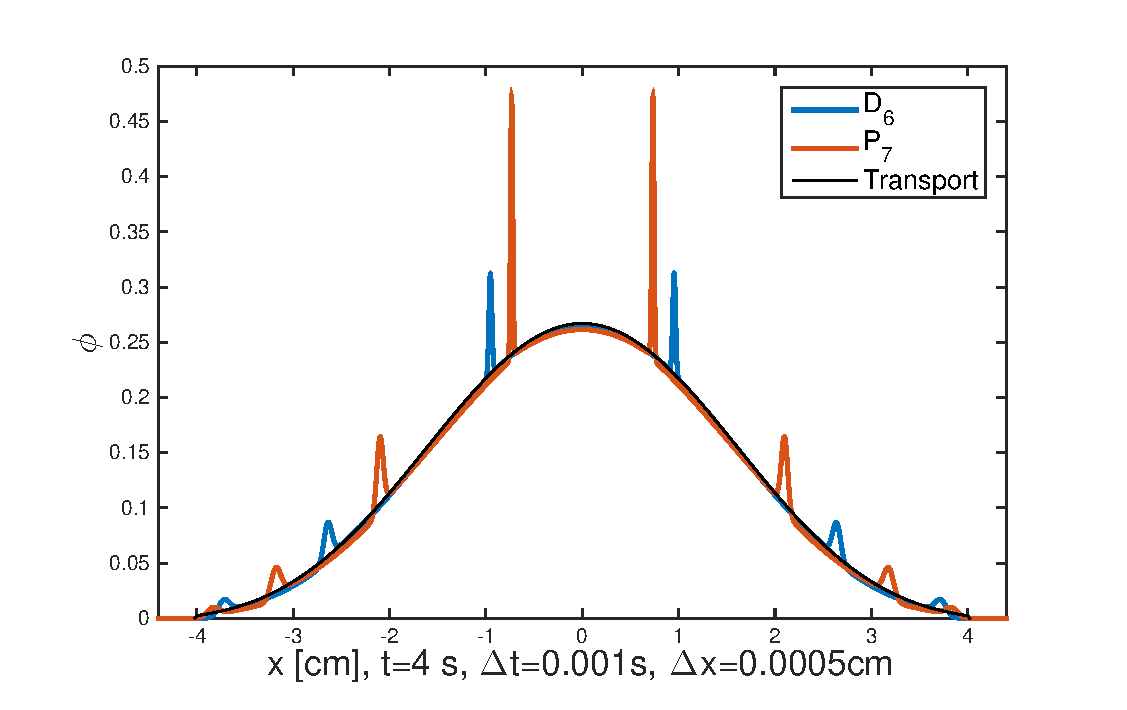
\includegraphics[width=8cm,height=4.8cm]{bd0_4s.eps}
		\includegraphics[width=1.\linewidth]{bd0.pdf}
		\caption{Solutions at an earlier time ($t=4$)}
		\label{f:bd0}
	\end{subfigure}
	\caption{Examples of \pn\ and \dn\ in plane source problem. Notice that early in time the discrete wave speeds in the \pn and \dn~solutions.}
	
\end{figure}

{
In the solution at earlier times (see Fig.~\ref{f:bd0}) there are spikes that are the numerical representation of waves of uncollided particles. Since the time dependent \pn\ system is a hyperbolic wave equation system, particles moves in several discrete wave speeds. The consequence is that the solutions will have $N+1$~spikes,~analytically represented by a Dirac delta function. These artifacts from the \pn\ (and \dn) discretization are known as wave effects\cite{brunner_app_rad_trans}.
	}

\subsubsection{Comparison of ML\dn\ and linear closures}
In the results below, unless otherwise noted, we use a value of $\alpha = 2/3$. Later, we discuss this choice.

In Figure  \ref{mls} we compare MLD and the diffusive closure on the plane source problem. At an early time, Figure \ref{f:mld4}, the wave effects are greatly reduced in the MLD$_6$ model relative to D$_6$\ and P$_7$.\ Furthermore, the solution away from the waves is much closer to the transport solution. At later time, Figure \ref{f:mld6}, the wave effects in P$_7$ and D$_6$ are still present whereas the MLD$_6$ solution has the overall shape of the transport solution with small oscillations near the D$_6$ waves. 

\begin{figure}[ht!]
	\begin{subfigure}{.5\textwidth}
		\centering
		%		\hspace*{-3cm}\includegraphics[width=8cm,height=5cm]{gd0_10s.eps}
		\hspace*{-1cm}\includegraphics[width=1.\linewidth]{ml6_1s2.pdf}
		\caption{MLD$_6$\ results at 1s in plane source problem.}
		\label{f:mld4}
	\end{subfigure}
	~
	\begin{subfigure}{.5\textwidth}
		\centering
		%\hspace*{-0cm}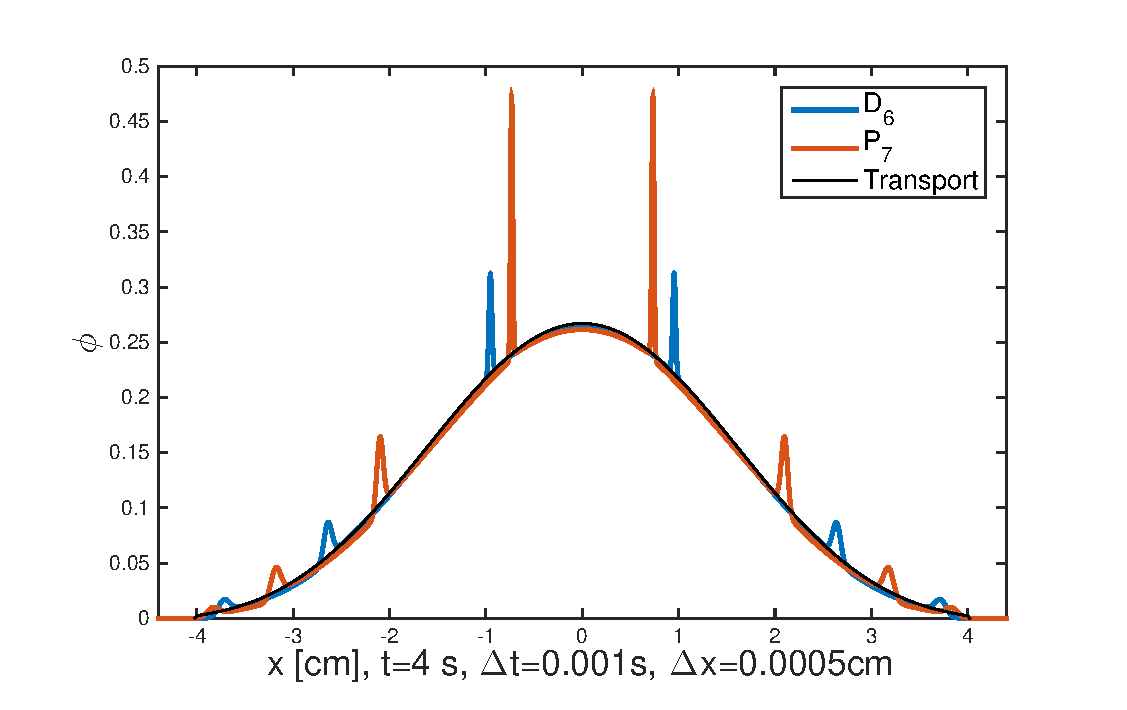
\includegraphics[width=8cm,height=4.8cm]{bd0_4s.eps}
		\includegraphics[width=1.\linewidth]{ml6_3s2.pdf}
		\caption{MLD$_6$\ results at 3s in plane source problem.}
		\label{f:mld6}
	\end{subfigure}
	\caption{ML\dn~and linear closure~solutions to the plane source problem at different times.}
	\label{mls}
\end{figure}
%\begin{figure}
%	\centering
%	%\hspace*{-0cm}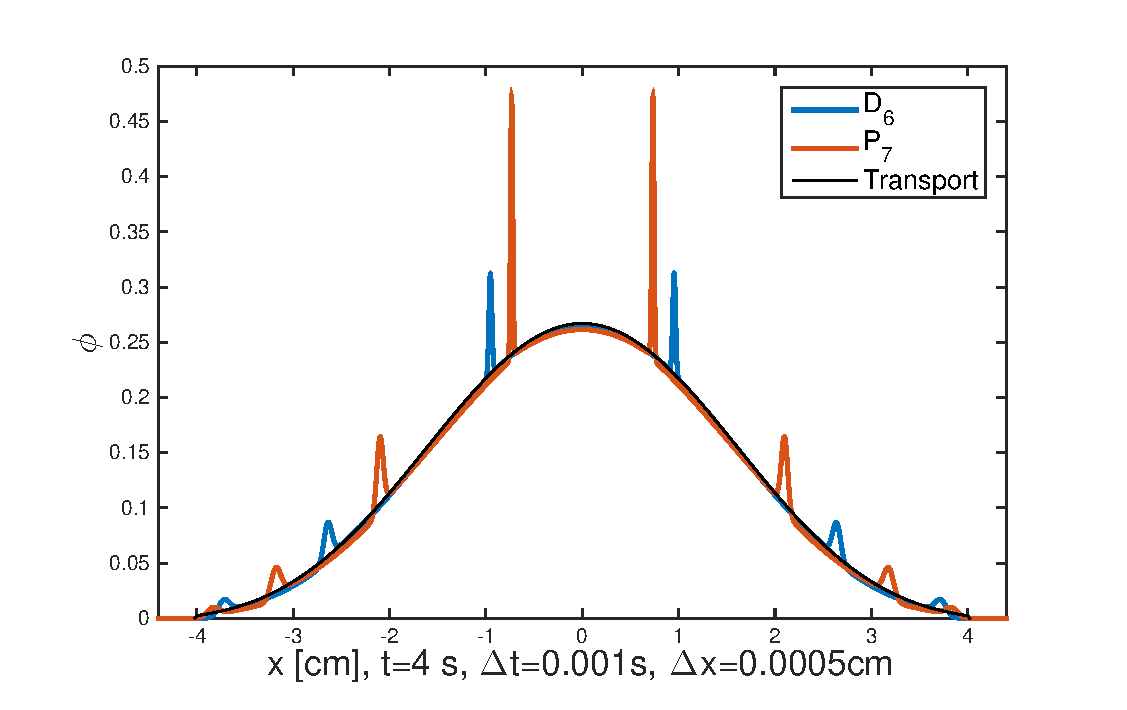
\includegraphics[width=8cm,height=4.8cm]{bd0_4s.eps}
%	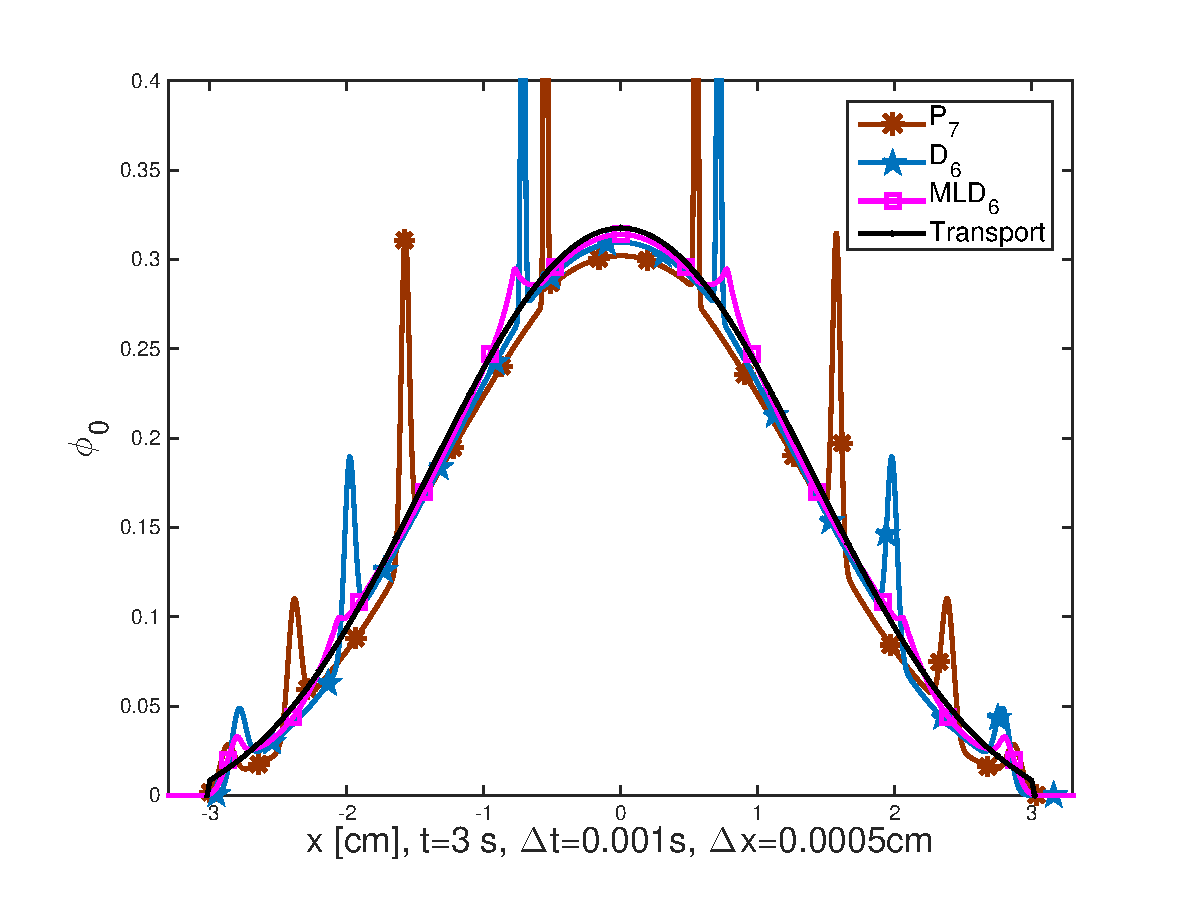
\includegraphics[width=1\linewidth]{ml6_3s.eps}
%	\caption{Artificial solutions.}
%	\label{ml6_3s}
%	\end{figure}

\subsubsection{Comparison of ML\dn\ and \tp{N}}
We next compare the two models developed in this paper.  At $t = 1$s\ in the plane source problem, as shown in Figure \ref{mlfls}, with both $N=6$ and $8$, the T\pn~model gives results closer to the transport solution than the ML\dn~model. %Additionally, near $x=0$ the MLD$_6$ and MLD$_8$ solutions are worse than the MLD$_4$ result from above.  

\begin{figure}[ht!]
	\begin{subfigure}{.5\textwidth}
		\centering
		%		\hspace*{-3cm}\includegraphics[width=8cm,height=5cm]{gd0_10s.eps}
		\hspace*{-1cm}\includegraphics[width=1.\linewidth]{ml_fl6_1s2.pdf}
		\caption{MLD$_6$\ and TP$_6$\ results.}
		\label{f:mlfl7}
	\end{subfigure}
	~
	\begin{subfigure}{.5\textwidth}
		\centering
		%\hspace*{-0cm}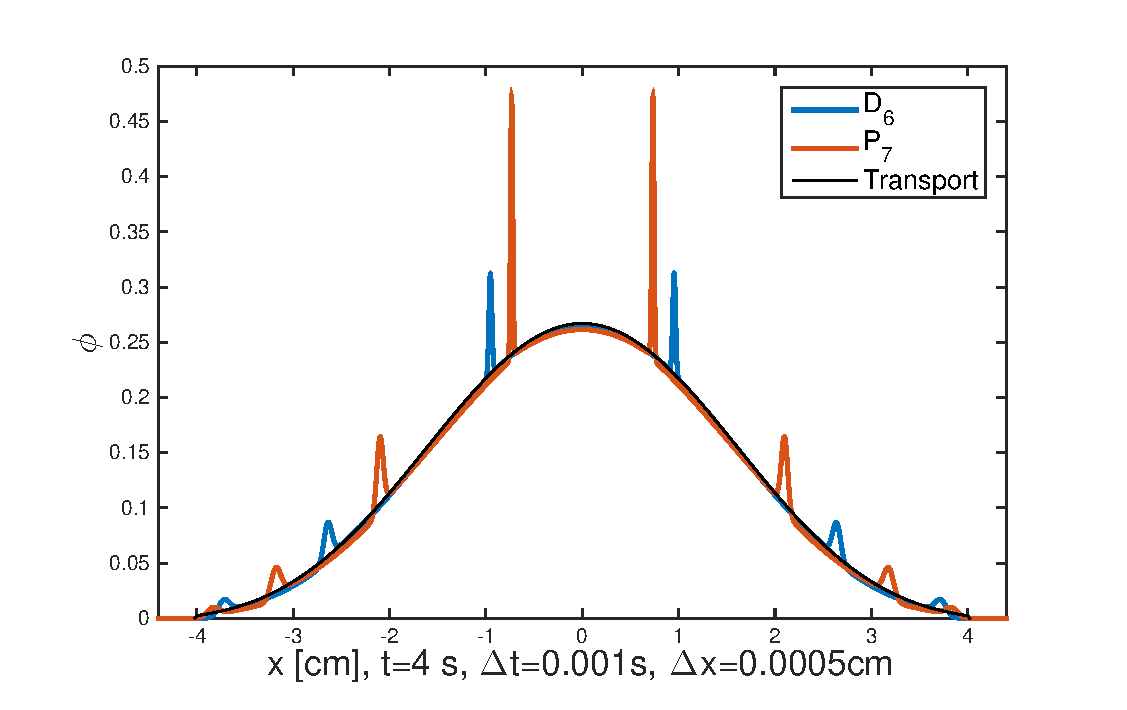
\includegraphics[width=8cm,height=4.8cm]{bd0_4s.eps}
		\includegraphics[width=1.\linewidth]{fl9_ml2.pdf}
		\caption{MLD$_8$\ and TP$_8$\ results.}
		\label{f:mlfl9}
	\end{subfigure}
	\caption{ML\dn\ and T\pn\ comparison at 1 s.}
	\label{mlfls}
\end{figure}

At 5s after the pulse, it is seen that in Figure\ \ref{mlfls2},\ both closures do not produce artificial waves in the solution to the degree that \dn~or \pn~solutions do. The  MLD$_N$\ and TP$_N$\ results basically agree to the transport solution in the middle except the solution near the wavefronts in the $\pm 5$\ cm. At the wavefront none of these methods captures the solution correctly.
\begin{figure}[ht!]
	\begin{subfigure}{.5\textwidth}
		\centering
		%		\hspace*{-3cm}\includegraphics[width=8cm,height=5cm]{gd0_10s.eps}
		\hspace*{-1cm}\includegraphics[width=1.\linewidth]{fl3_comp_5s.pdf}
		\caption{MLD$_2$\ and TP$_2$\ results.}
		\label{f:flml3}
	\end{subfigure}
	~
	\begin{subfigure}{.5\textwidth}
		\centering
		%\hspace*{-0cm}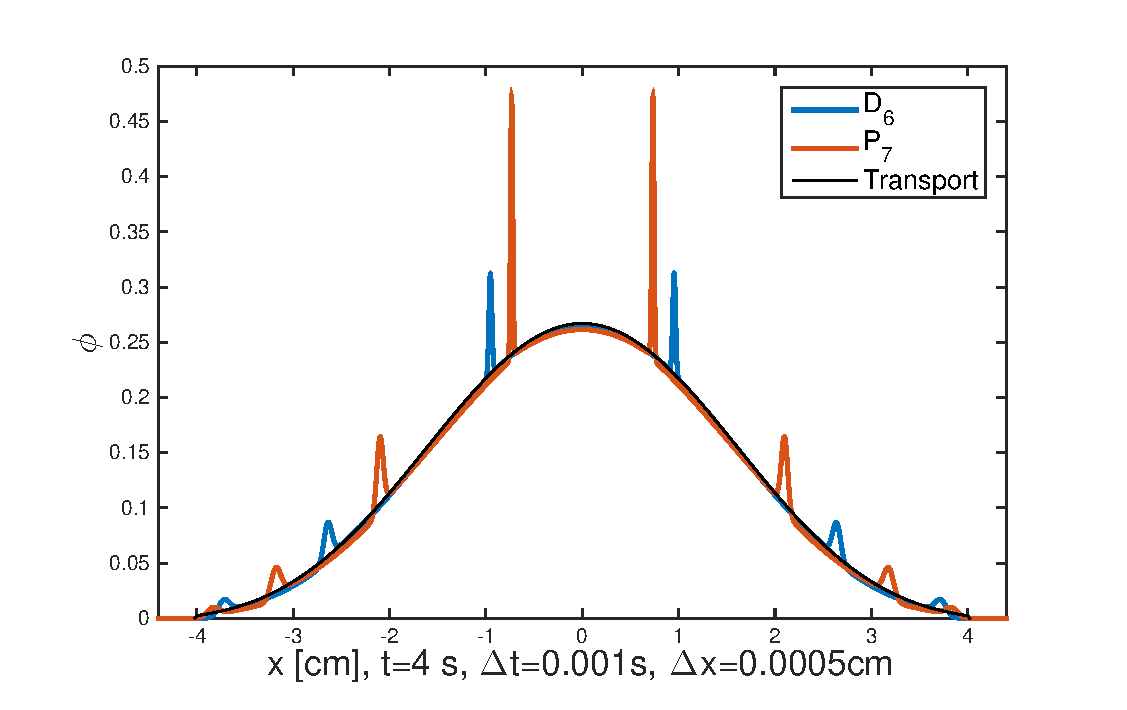
\includegraphics[width=8cm,height=4.8cm]{bd0_4s.eps}
		\includegraphics[width=1.\linewidth]{fl5_comp_5s.pdf}
		\caption{MLD$_4$\ and TP$_4$\ results.}
		\label{f:flml5}
	\end{subfigure}
	\caption{ML\dn\ and T\pn\ comparison at 5s.}
	\label{mlfls2}
\end{figure}
In summary, both the ML\dn~and T\pn\ closures effectively damp the unphysical modes (large spikes), which leads to relatively accurate solutions for the transport problem during short-time transients. Moreover, on every problem we have tested, the T\pn~ method was superior to the ML\dn~method.  Henceforth, we will focus on this method. 


%\subsection{The impact of the derivative terms}
%\subsubsection{Comparison with P$_N$ (even N)}
%\begin{figure}[ht!]
%	\begin{subfigure}{.5\textwidth}
%		\centering
%		%		\hspace*{-3cm}\includegraphics[width=8cm,height=5cm]{gd0_10s.eps}
%		\hspace*{-3cm}\includegraphics[width=1.4\linewidth]{p2_main.pdf}
%		\caption{TP$_2$\ compared with P$_2$\ results.}
%		\label{f:p2}
%	\end{subfigure}
%	~
%	\begin{subfigure}{.5\textwidth}
%		\centering
%		%\hspace*{-0cm}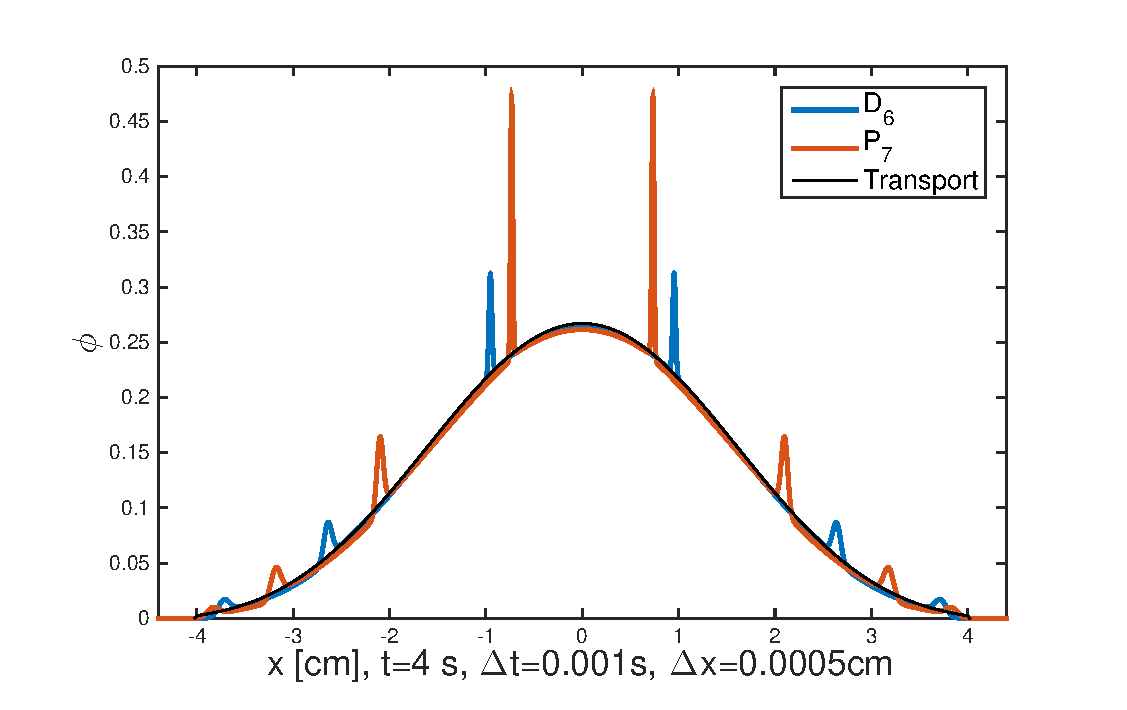
\includegraphics[width=8cm,height=4.8cm]{bd0_4s.eps}
%		\includegraphics[width=1.43\linewidth]{p8_main.pdf}
%		\caption{TP$_8$\ compared with P$_8$\ results.}
%		\label{f:p8}
%	\end{subfigure}
%	\caption{ML\dn\ and T\pn\ comparison at 1s.}
%	\label{f:evenpn}
%\end{figure}
%
%It shall be noticed that the two nonlinear closures in this papers are used with even order \pn. That is $N$ is an even number. In such a setting, one then can archive the rotational invariance without extra treatment on boundary condition. In practice, former work indicates that even order \pn\ in 1D has a static mode which never moves when wave effects of \pn\ approximation manifests \cite{mccdissertation,brunner_2d_pn}.\ As shown in Figure\ \ref{f:evenpn},\ the static mode stays in slab center. A lot of particles are stored in the middle and wait for collision.
%
%With \dn's treatment, however, the static mode is totally dampened. However, it does not effectively either retain the magnitude of the main mode in the slab center or dampen all other artificial modes. In fact, since the eigenstructure of the Jacobian is changed, the main effect is the speed change.
%
%Nevetheless, \tp{N}\ closure recovers more accurate flux profile than the \dn\ while effectively wiping artificial waves out.

\subsubsection{The impact of spatial and temporal terms in the model}
\begin{figure}[ht!]
	\begin{subfigure}{.5\textwidth}
		\centering
		%		\hspace*{-3cm}\includegraphics[width=8cm,height=5cm]{gd0_10s.eps}
		\hspace*{-1cm}\includegraphics[width=1.\linewidth]{fl3_limiters_1s2.pdf}
		\caption{TP$_2$ results at $t = 1$ s}
		\label{f:fl3limiter}
	\end{subfigure}
	~
	\begin{subfigure}{.5\textwidth}
		\centering
		%\hspace*{-0cm}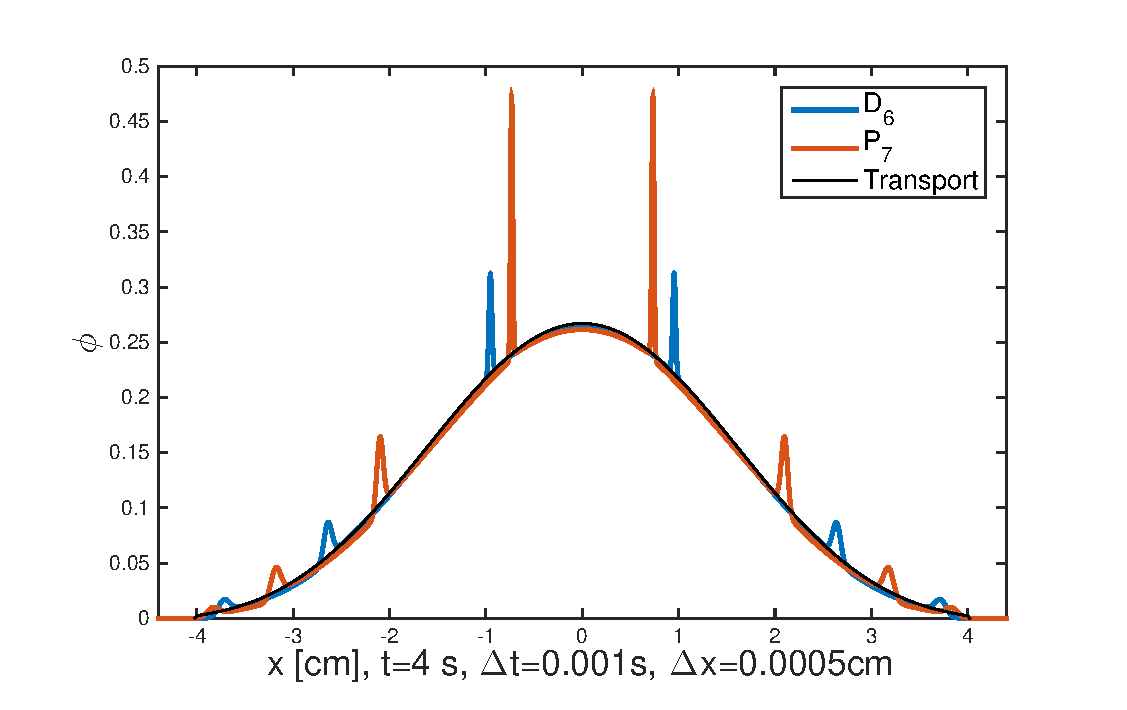
\includegraphics[width=8cm,height=4.8cm]{bd0_4s.eps}
		\includegraphics[width=1.\linewidth]{fl3_limiters_3s.pdf}
		\caption{TP$_2$ results at $t = 3$ s}
		\label{f:fl5limiter}
	\end{subfigure}
	\caption{Illustration of the impact of the spatial and temporal derivative terms in the T\pn~closure.}
	\label{f:limiters}
\end{figure}

To further investigate the importance of different terms in the closure, we individually turn on/off different derivatives in the closure. It is observed that, at 1\ s in the plane source problem in Figure \ref{f:fl3limiter} using only the spatial derivative term in the closure makes the solution flat in the middle and, as a result, too low. On the other hand, merely using the temporal derivative terms retains a better flux profile in the slab center, while the artificial spikes are not yet dampened effectively as with spatial limiter at later times in Figure \ref{f:fl5limiter}. Note that the moving modes propagate further than those with the spatial limiter. Therefore, we conclude that both derivative terms in the closure contribute to the accuracy of the model. %In addition, it also leads to fast convergence of T\pn\ model to transport solution in the graph norm.

%With time flying by, though all T\pn\ results retains better agreement than \dn\ with the transport solution, the mixed use of two limiters does bring in better dampening of the artificial solution discountinuity as shown in the zoomed figure in Figure\ \ref{f:fl5limiter}.

\subsubsection{Impact from Power $n$\ of T\pn\ models}
 It is observed that for low order T\pn\ approximations, varying the power $n$ does adjust the dissipation in the solution. As illustrated in Figure\ \ref{f:tp3n}, the originally proposed value, $n=1$\ retains the correct value near $x=0$. Simultaneously, $n=2$\ makes the solution flatter. On the other hand, reducing $n$\ to $1/3$ amplifies the dampened spikes and makes the solution more similar to the even \pn\ flux profile in that it has a stationary mode at $x=0$. It would suggest small powers should be avoided. Yet, all solutions agree with each other when the transient is passed.
We have also observed that with increasing $N$\ the solution becomes less sensitive to the power $n$ for $n>1$.


\begin{figure}[ht!]
%	\begin{subfigure}{.5\textwidth}
%	\centering
%	%		\hspace*{-3cm}\includegraphics[width=8cm,height=5cm]{gd0_10s.eps}
%	\hspace*{-3cm}\includegraphics[width=1.4\linewidth]{fl5coef_2s.pdf}
%%	\caption{1TP$_2$\ compared with P$_2$\ results.}
%	\label{f:tp2coef}
%\end{subfigure}
%~
%\begin{subfigure}{.5\textwidth}
\centering
%\hspace*{-0cm}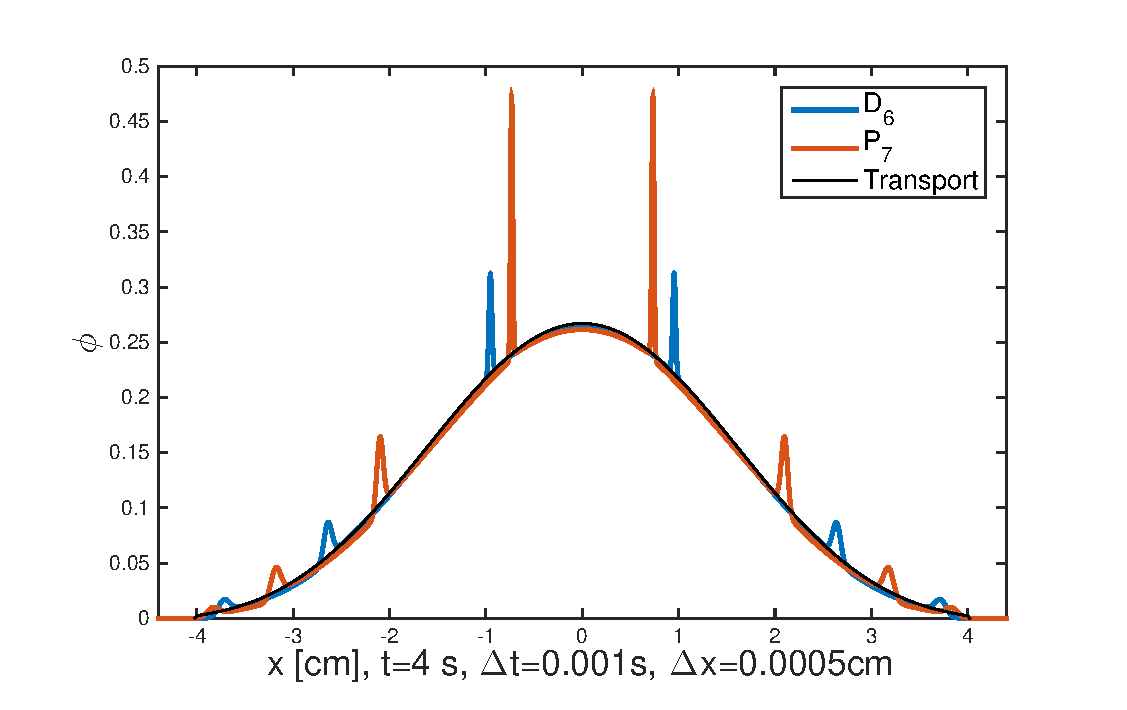
\includegraphics[width=8cm,height=4.8cm]{bd0_4s.eps}
\includegraphics[width=.5\linewidth]{fl3_n_comp2.pdf}
\caption{Effects from different power $n$ on the in Eq.~(\ref{eq:fluxLim}).}
\label{f:tp3n}
%\end{subfigure}
%\caption{ML\dn\ and T\pn\ comparison at 1s.}
%\label{f:coef}
\end{figure}
\subsubsection{Spatial derivative coefficient $\alpha$}
In our initial derivation of the T\pn~model we surmised that the value of $\alpha$ should be between $1/3$ and 1 because it appears in a similar way to the coefficients of the \pn~Jacobian. Since these coefficients range from $1/3$ through 1, we therefore used the median value $2/3$. %We initially expected this choice would introduce the dissipation more reasonably since we somehow add the information of the speed of information transmission into the closure. 

%On the other hand, \dn's treatment on assuming the closed moment to be static is more like admitting an infinite-speed mode in the solution. Consequently, the static mode in even order \pn\ is dissipated at very early time after imposing the pulse in the plane source problem, which also leads to over-diffusive result in short-time transient limit in our observations.

We present a limited parameter study for $\alpha$  in Figure\ \ref{f:tp6coef}. Therein, the flux profiles vary in several respects. With the smallest value shown, $\alpha=1/3$, the solution is much closer to the \dn~solution: the solution is too low in the middle, and the wave effects are amplified. On the other hand, increasing $\alpha$\ to 1 appears to amplify and spread the waves in the solution in addition to increasing the solution near $x=0$ too much.

Compared with 1/3 and 1, $2/3$\ provides the most accurate and least oscillatory result among the three choices. We have performed more  studies using many more values of $\alpha$ and found that  $\alpha$ values of 0.5 through 0.7 are comparable to the 2/3 solution.

\begin{figure}[ht!]

	\centering
	%\hspace*{-0cm}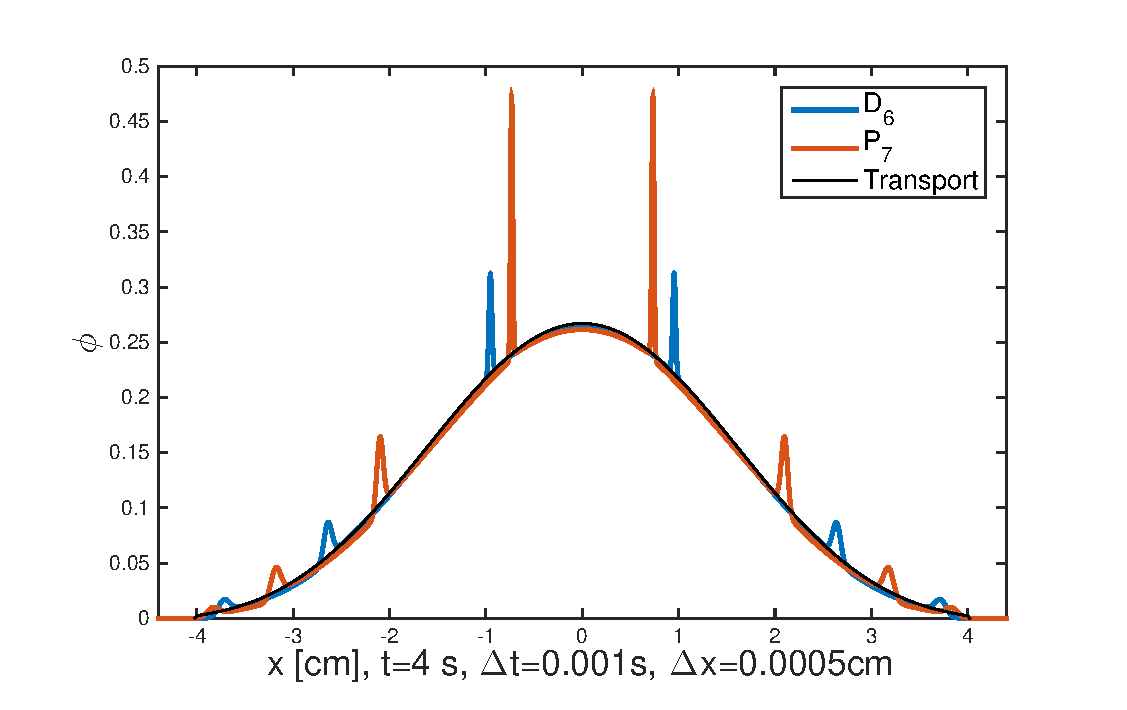
\includegraphics[width=8cm,height=4.8cm]{bd0_4s.eps}
	\includegraphics[width=.5\linewidth]{fl7coef_1s.pdf}
	\caption{Effects from different coefficients $\alpha$ in the closure. With $\alpha =0 $ the spatial derivative of the scalar flux has no impact on the closure.}
	\label{f:tp6coef}
\end{figure}



\subsection{Two-beam problem}

\begin{figure}[ht!]
	\begin{subfigure}{.5\textwidth}
		\centering
		\hspace*{-1cm}\includegraphics[width=1.\linewidth]{tp2_bru.pdf}
		%\caption{P$_3$QT time-dependent solution}
		%\label{bmtrhort}
	\end{subfigure}
	~
	\begin{subfigure}{.5\textwidth}
		\centering
		\includegraphics[width=1.\linewidth]{d2_bru.pdf}
		%\caption{P$_3$QS (D$_2$) time-dependent solution}
		%\label{gptrhort}
	\end{subfigure}
	\caption{Comparison between TP$_2$ and D$_2$\ (P$_3$QS) solutions to two-beam problem.}
	\label{exp}
\end{figure}

The second test problem is a highly absorbing problem with isotropic incident angular fluxes on both sides of a slab. The scattering ratio, $c=\sigmas/\sigmat$,~of the medium is $0.1$. The original test problem is in steady state\cite{brunnerentropy}.\ We, however, run this problem in time-dependent mode to see how different methods approach the steady state solution. These results are shown in Figure\ \ref{exp}.

Both \tp{N}\ and \dn\ converge to the reference solution at 10\ s. Theoretically, incident particles from different sides of the slab are not supposed to meet before $t=L/(2v)=5$\ s. Yet, D$_2$\ artificially moves particles faster than their physical speeds, making the solution greater than $10^{-8}$ at $x=0$ as early as $t=2$s.  On the other hand, the TP$_2$\ model retains a sharper wavefront and as a result the solution at $x=0$ is below $10^{-8}$ until 5 s. 

Though the incident flux is isotropic on the boundary, the angular flux gradually turns to become strongly anisotropic and form a beam-like distribution in the middle of the slab due to the strong absorption. This beam-like behavior of the angular flux is a potential challenge for the model. Some closure models, such as the entropy based closure model (M$_N$),~have difficulty in resolving the beam. For the M$_N$~method, it tends to have artificial shock in the middle (Ref.~\cite{coryentropy,brunnerentropy}).~It is also suspected in Ref.~\cite{coryentropy}~that this shock could possibly caused by small errors when solving minimization problem governing the M$_N$~method. Fortunately, the TP$_{N}$~model does not have the artificial shock in this problem.
%\subsection{Limiter effects on wavefront}
%Basically discuss Figure~\ref{exp}.
%
%The T\pn\ model, having a similar form as D$_N$~model, automatically add nonlinear dissipation to the highest moment. Since the simulation in the double-incident problem is performed in a time-dependent way, a physical solution should preserve the property that before $t=L/(2v)$,~fluxes propagated from different incidents, shall not contact each other because the particle should not have a speed over $v$.
%
%However, as shown in Figure~\ref{exp},~P$_3$QS (D$_2$)~over diffuses the particles such that the fluxes from different sides get contacted, which is like artificially accelerating the particles. Compared with this diffusive closure model, P$_3$QT, yet, somehow, limits the accelerations, which preserves very sharp wavefront.
%\begin{figure}[ht!]
%\centering
%\subfigure[P$_3$QT]{0.5\textwidth}
%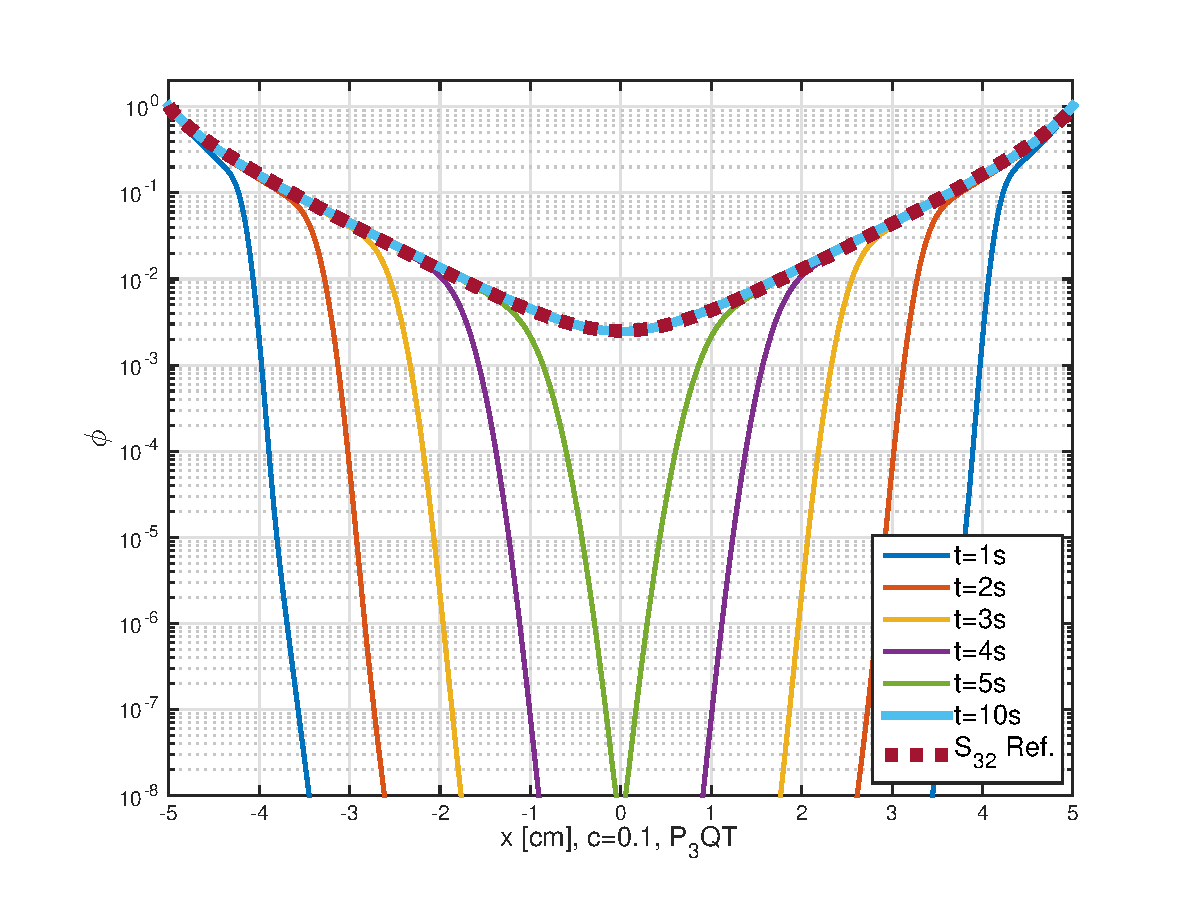
\includegraphics[width=0.9\linewidth]{brunner_p3qt.eps}
%\caption{Parameter significances (mean sums of squares) from ANOVA analysis.}
%\label{fg:anova_sig}
%\end{subfigure}
%~
%\begin{subfigure}{0.5\textwidth}
%\centering
%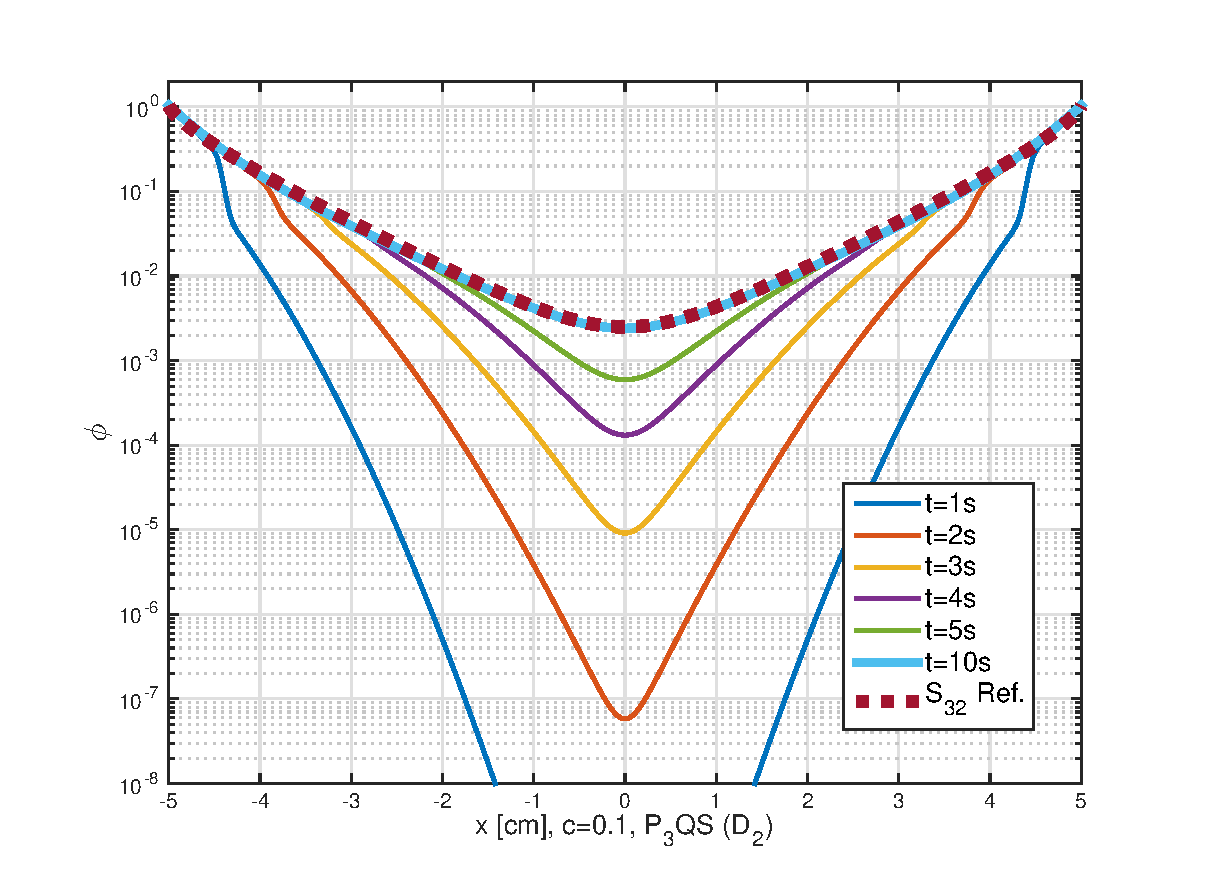
\includegraphics[width=0.9\linewidth]{brunner_p3qs.eps}
%\caption{Parameter significances (relative relevance) from GPR emulation.}
%\label{fg:gpr_sig}
%\end{subfigure}
%\caption{Parameter significance comparisons from different methods.}
%\label{fg:sigs}
%\end{figure}



%\begin{figure}[ht]
%\centering
%\begin{minipage}[b]{0.5\linewidth}
%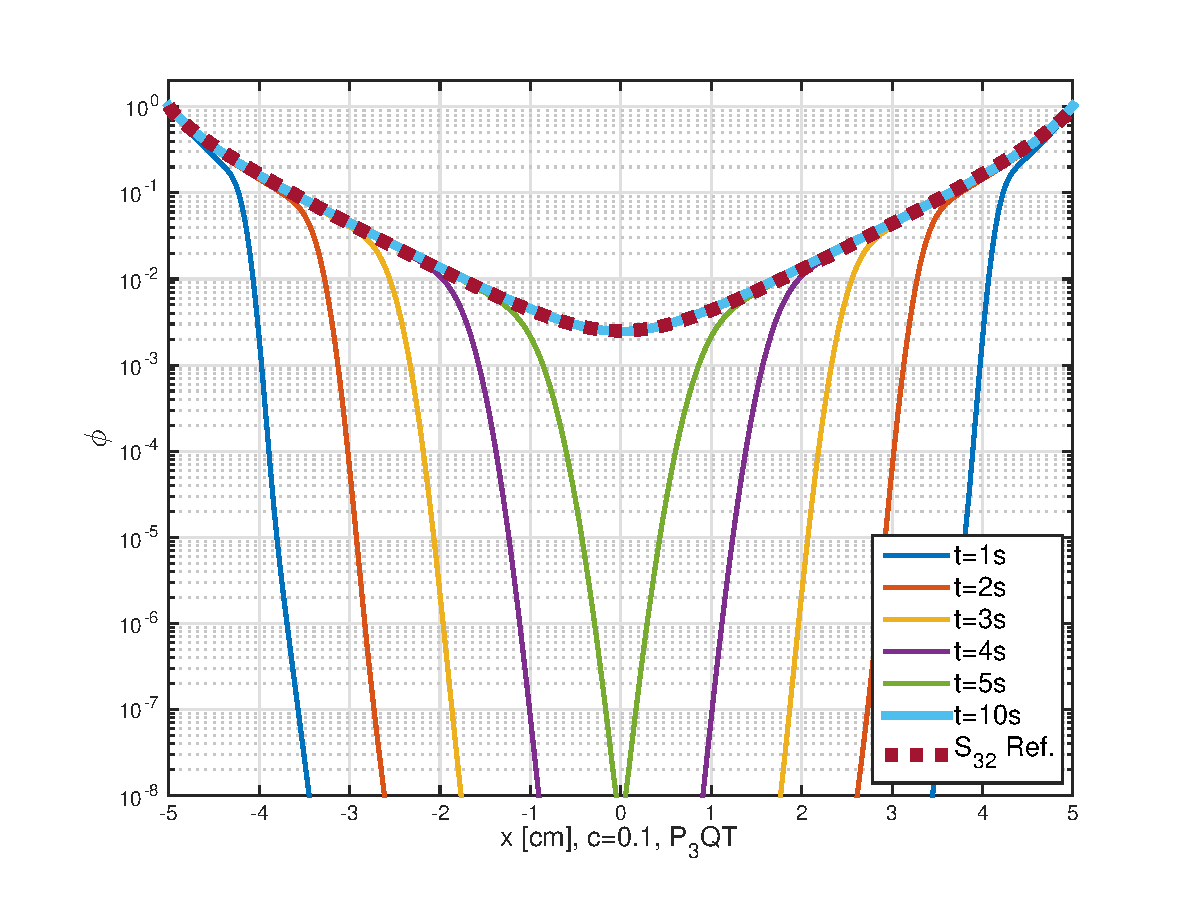
\includegraphics[width=0.19\linewidth]{brunner_p3qt.eps}
%\caption{Happy Smiley}
%\label{fig:minipage1}
%\end{minipage}
%\begin{minipage}[b]{0.5\linewidth}
%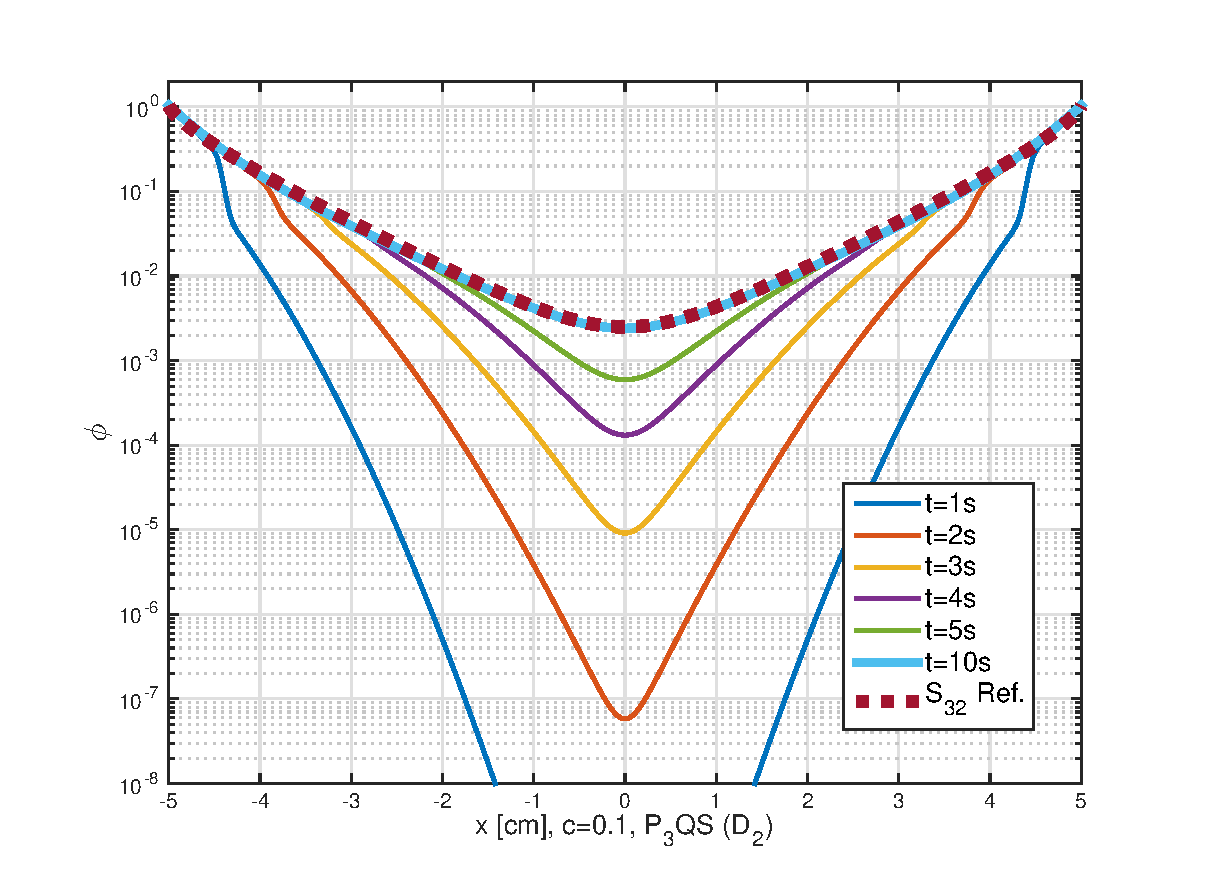
\includegraphics[width=0.19\linewidth]{brunner_p3qs.eps}
%\caption{Sad Smiley}
%\label{fig:minipage2}
%\end{minipage}
%\end{figure}


%\subsubsection*{Boundary condition test}

\subsection{Reed's problem}
The last test problem in this work is  Reed's problem \cite{reed_1971}. It contains several regions with largely varied properties including strong pure absorbers, voids, strong source and material discontinuities.

The numerical example in Figure~\ref{reed2}~is TP$_4$\ and D$_4$\ solutions of Reed's problem. In voids, in order to make the diffusive closure well-posed, an artificial absorption $\zeta$ is chosen:
\begin{equation}
	\st'=\st+\zeta, %\delta(\st),
\end{equation}
where $\zeta$~is a small number, which is fixed at $10^{-8}$. For the TP$_N$\ model we only need a correction when $\tilde\sigma$ is zero, (i.e., in voids when then the scalar flux is constant in space and time). The correction we use is
\begin{equation}\label{tp}
\tilde{\sigma}'=\tilde{\sigma}+\zeta, %\delta(\tilde{\sigma}).
\end{equation}

\begin{figure}[ht!]
	\begin{center}
		\includegraphics[width=.5\textwidth]{reed_tp4_d4_d6.pdf}
		%\includegraphics[width=0.45\textwidth]{srholam.eps}
		\caption[]{Reed's problem solved with D$_4$,\ TP$_4$,\ and D$_6$\ compared with S$_{32}$.}% Only the ``Figure" label and figure number are bold.}
		\label{reed2}
	\end{center}
\end{figure}

We use $800$\ cells in the discretization for D$_4$,\ D$_6$,\ and \tp{4}.\ 
The  S$_N$\ solutions are calculated with cell centered difference  using 16,000\ cells. We observe that TP$_4$\ retains an accuracy comparable to D$_6$\ and S$_8$. As a comparison, D$_4$\ displays comparable accuracy to S$_6$.\ Given that in 1-D slabs, S$_{N+1}$ gives identical solutions to P$_N$, this result is evidence that the \dn~and T\pn~models improve the solution as indicated by our residual analysis. As our analysis also predicts, the T\pn~solution is superior to both \dn~and \pn.
% This would imply additional dissipation made by the flux limiters helps reduce the residual and improve the accuracy of the \pn\ system.

\begin{figure}[ht!]
	\begin{subfigure}{.5\textwidth}
	\begin{center}
		\hspace*{-1cm}\includegraphics[width=1.\textwidth]{reed_error12.pdf}
		%\includegraphics[width=0.45\textwidth]{srholam.eps}
		\caption[]{Pointwise absolute errors of D$_4$,\ TP$_4$,\ and D$_6$\ methods (Part 1).}% Only the ``Figure" label and figure number are bold.}
		\label{reed_er1}
	\end{center}
\end{subfigure}
~
\begin{subfigure}{.5\textwidth}
	\begin{center}
		\includegraphics[width=1.\textwidth]{reed_error22.pdf}
		%\includegraphics[width=0.45\textwidth]{srholam.eps}
		\caption[]{Pointwise absolute errors of D$_4$,\ TP$_4$,\ and D$_6$\ methods (Part 2).}% Only the ``Figure" label and figure number are bold.}
		\label{reed_er2}
	\end{center}
\end{subfigure}
\caption[]{\label{reed_error}Errors as a function of space in Reed's problem.}
\end{figure}

{Overall, as illustrated in Figure\ \ref{reed_error},\ the pointwise errors from TP$_4$\ are comparable to D$_6$\ and  smaller than those from D$_4$\ method in most regions especially for regions with large errors ($>10^{-2}$). We also observe that the boundary treatment in Eq~\eqref{e:bdy}\ brings about 0.8\% of error, slightly higher than D$_4$.\ However, the global $L_1$ norm of error for D$_4$ (estimated based on the fine-mesh S$_{32}$\ solution) is $0.129$\ and is larger than that of TP$_4$,\ which is $0.061$.\ For comparison, the D$_6$\ solution has an error of $0.066$.}

%{Note that in void region, since \dn\ takes the constant artificial cross section, the scalar flux is a constant, resulting in a constant error around 0.3 \%.\ Yet, the limiters in the closure of T\pn\ leads to non-constant smaller errors in such a region as illustrated in Figure\ \ref{reed_er1}.}
\subsection{2D line source problem}
\begin{figure}[ht!]
	\begin{subfigure}{.5\textwidth}
		\centering
		%		\hspace*{-3cm}\includegraphics[width=8cm,height=5cm]{gd0_10s.eps}
		\hspace*{-1cm}\includegraphics[width=1.\linewidth]{linesrc-ref.png}
		\caption{Analytic transport}
		\label{f:trans}
	\end{subfigure}
	~
	\begin{subfigure}{.5\textwidth}
		\centering
		%\hspace*{-0cm}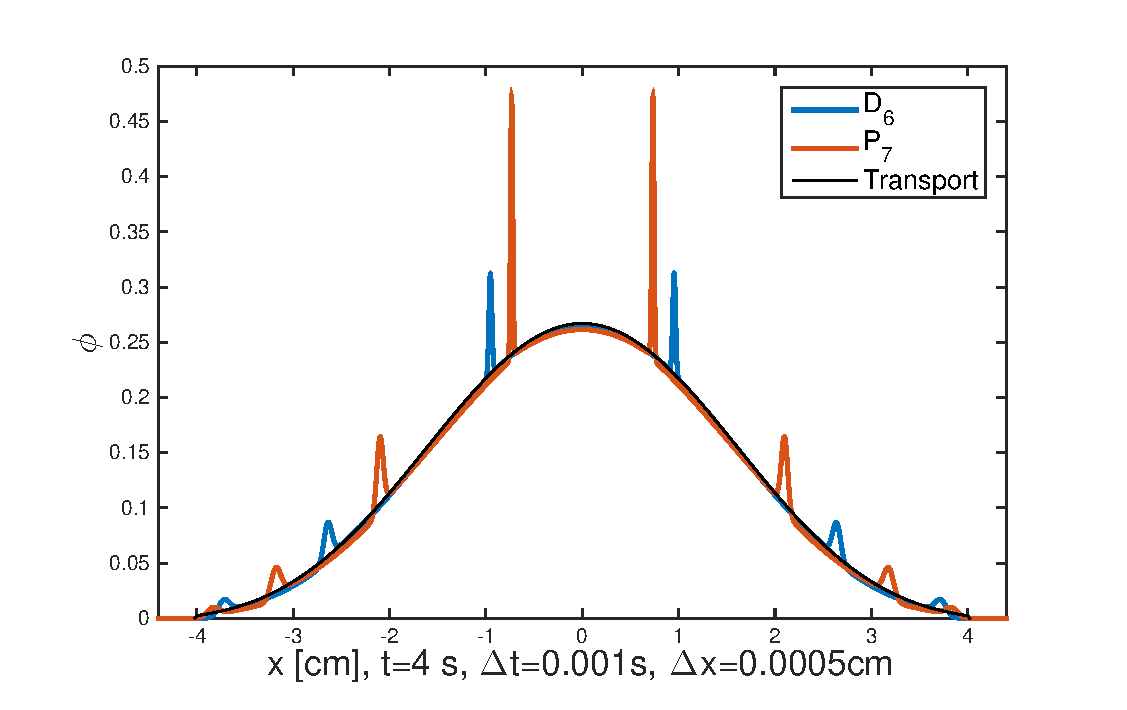
\includegraphics[width=8cm,height=4.8cm]{bd0_4s.eps}
		\includegraphics[width=1.\linewidth]{line-s8}
		\caption{S$_8$}
		\label{f:s8}
	\end{subfigure}
	~
	\begin{subfigure}{.5\textwidth}
		\centering
		%		\hspace*{-3cm}\includegraphics[width=8cm,height=5cm]{gd0_10s.eps}
		\hspace*{-1cm}\includegraphics[width=1.\linewidth]{p7.pdf}
		\caption{P$_7$}
		\label{f:p7}
	\end{subfigure}
	~
	\begin{subfigure}{.5\textwidth}
		\centering
		%\hspace*{-0cm}\includegraphics[width=8cm,height=4.8cm]{bd0_4s.eps}
		\includegraphics[width=1.\linewidth]{d6.pdf}
		\caption{D$_6$}
		\label{f:d6}
	\end{subfigure}
	~
	\begin{subfigure}{.5\textwidth}
		\centering
		%		\hspace*{-3cm}\includegraphics[width=8cm,height=5cm]{gd0_10s.eps}
		\hspace*{-1cm}\includegraphics[width=1.\linewidth]{tp2.pdf}
		\caption{TP$_2$}
		\label{f:tp2}
	\end{subfigure}
	~
	\begin{subfigure}{.5\textwidth}
		\centering
		%\hspace*{-0cm}\includegraphics[width=8cm,height=4.8cm]{bd0_4s.eps}
		\includegraphics[width=1.\linewidth]{tp-6.pdf}
		\caption{TP$_6$}
		\label{f:tp6}
	\end{subfigure}
	\caption{2D line source problem at $t=1$\ s.}
	\label{f:line}
\end{figure}
{
The line source problem is a 2D variation of the plane source problem in 1D slab geometry. The problem is an infinite, pure scattering medium ($\st=\sigmas=1$) with no source. The initial condition is given by\cite{ganapol}:
	\begin{equation}
	\psi(x,z,\hat{\Omega},0)=\frac{\delta(x)\delta(z)}{4\pi}
	\end{equation}
\pn,\ \dn\ and T\pn\ results in Figure\ \ref{f:line}\ are achieved with $\Delta t=0.02$\ s and $\Delta x=0.02$\ cm and S$_8$\ result is achieved from Ref.\ \cite{mccfpn09}.\ The analytic solution is shown in Figure\ \ref{f:trans}\ from the benchmark code AZURV1\cite{ganapol}.\ The wavefront at $r=\sqrt{x^2+z^2}=vt$,\ essentially a moving delta function, will induce oscillations and negative scalar fluxes in \pn\ and \dn\ methods as illustrated in Figures\ \ref{f:p7}\ and \ref{f:d6}.\ Meanwhile, for this streaming dominated problem, \sn\ results have strong ray-effects as in Figure\ \ref{f:s8}.\ On the other hand, TP$_2$\ solution presents plausible results in Figure\ \ref{f:tp2}.\ Increasing the angular order to TP$_6$\ will further improve the solution as illustrated in Figure\ \ref{f:tp6}. }

{Unlike the 1D T\pn\ model, multi-D T\pn\ models for different angular orders do not have a single coefficient $\alpha$,\ therefore, the results shown in Figure\ \ref{f:line}\ are obtained with different coefficients. Figure\ \ref{f:tp-lines}\ presents the diagonal lineout plots of TP$_2$,\ TP$_4$\ and TP$_6$\ with different $\alpha$.\ Changing the $\alpha$\ for each angular order can effectively change the results, as observed in 1D. Unfortunately, the ``optimal" values for different angular orders are different, e.g. while $\alpha=0.1$\ would lead to relatively accurate TP$_2$\ results, the ``optimal" $\alpha$\ changes to $1/3$\ and $1.5$\ for TP$_4$\ and TP$_6$,\ respectively. This should be addressed in future work.
\begin{figure}[ht!]
	\begin{subfigure}{.5\textwidth}
		\begin{center}
			\hspace*{-1cm}\includegraphics[width=1.\textwidth]{tp2-line.pdf}
			%\includegraphics[width=0.45\textwidth]{srholam.eps}
			\caption[]{TP$_2$\ results with different $\alpha$.}% Only the ``Figure" label and figure number are bold.}
			\label{f:tp2-line}
		\end{center}
	\end{subfigure}
	~
	\begin{subfigure}{.5\textwidth}
		\begin{center}
			\hspace*{0cm}\includegraphics[width=1.\textwidth]{tp4-line.pdf}
			%\includegraphics[width=0.45\textwidth]{srholam.eps}
			\caption[]{TP$_4$\ results with different $\alpha$.}% Only the ``Figure" label and figure number are bold.}
			\label{f:tp4-line}
		\end{center}
	\end{subfigure}
	~
	\begin{subfigure}{.5\textwidth}
		\begin{center}
			\hspace*{-1cm}\includegraphics[width=1.\textwidth]{tp6-line.pdf}
			%\includegraphics[width=0.45\textwidth]{srholam.eps}
			\caption[]{TP$_6$\ results with different $\alpha$.}% Only the ``Figure" label and figure number are bold.}
			\label{f:tp6-line}
		\end{center}
	\end{subfigure}
	\caption[]{\label{f:tp-lines}Diagonal lineout plots for TP$_2$\ and TP$_6$.}
\end{figure}
	}

{
2D \pn,\ \dn\ and T\pn\ are solved with (semi-)implicit discretization in time and DG/LDG method in space. A GMRES solver is used with the Jacobi preconditioner. A comparison of timings for T\pn\ and linear closures is made in Table\ \ref{t:cpu_time}.\ Simulations were run on a Mac mini with Intel i7-3615 processor and 16GB 1600MHz DDR3 RAM.
}

{
With LDG method, \dn\ and T\pn\ have the same number of degrees of freedom (DoFs) as P$_{N+1}$\ with the same basis functions used on the same mesh. The overall CPU time of T\pn\ is much shorter than \dn.\ The hypothesis is that the \dn\ model sets the time dependence of $\phi_{N+1}^m$\ to be zero, forcing particles in that mode to move with infinite speed. This makes \dn\ model physically ill-posed in time dependent problems. Numerically, the ill-posedness causes the degradation of the preconditioning efficiency.
}

{
On the other hand, though TP$_2$'s\ solving time is around 73\%\ higher than P$_3$,\ TP$_6$'s\ solving time is comparable to P$_7$. The correction brought by flux limiters affects not only the physical properties as discussed in 1D scenarios, but also the computational properties. %A few percent extra cost caused by updating and reassembling limiters should be efficiently reducable with proper parallelization. 
Overall, we conclude T\pn\ would be comparably efficiently solved as \pn\ in multi-D applications.
\begin{table}[h]
	\centering
	\caption{Timings for line source problem at 1s.}
	\label{t:cpu_time}
	\begin{tabular}{|c|c|c|c|}
		%\label{tb:1}
		\hline
		& P$_3$ & TP$_{2}$ & D$_{2}$\\
		\hline
Setup+assembly time [s] & 6.9 & 7.4 & 7.2\\
\hline
		Estimate+assemble limiter time [s]& 0 & 16.5 & 0 \\
		\hline
		Solving+preconditioning time [s]& 124.6 & 215.6 & 562.8 \\
		\hline
		Total CPU time [s]& 131.5  & 228.5 & 570.0\\
		\hline
		\hline
		& P$_5$ & TP$_{4}$ & D$_{4}$\\
		\hline
Setup+assembly time [s] & 20.6  & 19.5 & 18.5\\
\hline
Estimate+assemble limiter time [s]& 0 & 28.3 & 0 \\
\hline
Solving+preconditioning time [s]& 383.5 & 482.0 &  1308.8\\
\hline
	Total CPU time [s]& 404.1 & 529.8 & 1327.3\\
		\hline
		\hline
		& P$_7$ & TP$_{6}$ & D$_{6}$\\
		\hline
		Setup+assembly time [s] & 43.7  & 42.4 & 43.0\\
		\hline
		Estimate+assemble limiter time [s]& 0 & 153.2 & 0 \\
		\hline
		Solving+preconditioning time [s]& 734.5 & 760.4 & 2424.7 \\
		\hline
		Total CPU time [s]& 778.1 & 956.0 & 2467.7\\
		\hline
	\end{tabular}
\end{table}
	}

\section{Concluding remarks}
%\subsection{Summary}
In this paper, we analyzed the effects on the \pn~approximation residual caused by different closures. We provide a new explanation of the reasons the conventional \pn~and \pn~with diffusive closure has issues in transient simulations, such as the pulsed plane source problem {in 1D and line source problem in 2D}. Based on the analysis, we proposed two novel closures, the ``moment-limited" closure for 1D and ``transient'' \pn\ closure in 1D and 2D. The results we presented indicate that, relative to other linear closures, our new closures perform better on a variety of problems, including the notorious plane source problem {and line source problem}. 
%\subsection{Future work}

{
%In 2D, T\pn\ does demonstrate the efficacy of adding flux limiters to the moment system to improve the solution. Futhermore, as the flux limiters have the same unit of a cross section, we would also interpret them as angular viscosity added to the \dn\ system. The fact motivates us to introduce the ``viscosity" to F\pn\ in the ongoing work.\ A favorable feature of such a F\pn\ method would be that the filtering strength would be automatically determined by the solution, differring from conventional F\pn\ method that the amount of viscosity needs to be fully determined by modelers with knowledge of the solution.
}

{
%Currently, estimation of the limiters for 2D is based on the cell center difference using rectangular mesh and therefore rather indirect for estimation to unstructured mesh. This should be addressed in the future work.
}
%We believe TP$_N$\ is a promising model and we are currently undertaking an extension to 2- and 3-D. In multi-dimensional problems it is possible that the T\pn~model removes the negative scalar fluxes that are possible in \pn~solutions. Theoretically, T\pn~could give positive solutions because it is a nonlinear closure as shown in previous studies \cite{McClarren:2008hu}. 

Finally, we believe that the ideas behind the T\pn~model could be used in other transport models. For instance, this type of closure could be applied to the simplified \pn~method \cite{McClarren:2011ga}. 
%{
%We further point out that the T\pn\ closure could be interpreted as adding angular viscosity, in forms of flux limiters, to the highest moments of \dn\ closure. This motivate us developing a nonlinear filtered \pn\ method as introduced in \cite{fpn_radice,mccfpn09}\ based upon such a ``viscosity". In contrast to the previously developed filtered \pn\ method that modelers should predefine the amount of viscosities based on the knowledge of solution, such a filter would determine the viscosity automatically nonlinearly in light of the solution.
%	}
%Also, in order to obtain high resolution with diamond differences, we set very fine mesh with small time steps, which is impractical for large systems and multi-D applications. 
%Also, the boundary treatment is not perfect from the Reed's problem result. Generally speaking, low-order T\pn\ results in slightly higher error than \dn\ method on the left boundary in Reed's problem. More investigations is worth performing on the boundary errors.

\section*{Acknowledgements}
The authors would like to thank the anonymous reviewers for their valuable comments and suggestions to improve the quality of the paper. W. Zheng would like to thank Dr.\ Wolfgang Bangerth from the Dept. of Mathematics at Texas A\&M University for helpful discussions about efficient implementations of the multi-D applications in deal.II. Also, W. Zheng is thankful to Dr.\ Robert Lowrie from Los Alamos National Laboratory for providing the LDG idea for multi-D application.

This project is funded by Department of Energy NEUP research grant from Battelle Energy Alliance, LLC- Idaho National Laboratory, Contract No: C12-00281.


\section*{References}
\bibliography{mybibfile}

\end{document}